\appendix
\phantomsection % To have a correct link in the table of contents
\addcontentsline{toc}{chapter}{Supplementary material}
\chaptermark{Supplementary material}

\topskip0pt
\vspace*{\fill}
\begin{center}
\Huge \textbf{Supplementary material} \normalsize
\end{center}
\vspace*{\fill}



\chapter{Statistical tools for spatial and spatio-temporal modeling}

\section{Properties of spatio-temporal covariance functions}\label{appendix:cov_prop}

\vspace{\baselineskip}

\underline{\textit{Non-negative and positive-definiteness}}

A function $\{\mathcal{C}(u,v):u,v\in D\}$ defined on $D \times D$ is said to be \textbf{non-negative-definite}, if for any complex numbers $\{a_i:i=1,...,m\}$, any $\{u_i:i=1,...,m\}$ in $D$, and any integer $m$, we have 

$$\sum^m_{i=1}\sum^m_{j=1}a_i \bar{a}_j \mathcal{C}(u_i,u_j) \geq 0$$

where $\bar{a}$ denotes the complex conjugate of $a$.

To be $valid$, a covariance function must be non-negative definite.

A function is \textbf{positive-definite} when the inequality below is strictly positive whenever $(a_1,...,a_m)'$ is a nonzero vector.

For the following properties, we rewrite $u$ as $u = (s;t)$ and $\mathcal{C}(u_i,u_j) \equiv \mathcal{C}((x_i,t_i),(x_j,t_j))$.

In our case as the time is assumed discrete, the domain $D$ is a subset of $\mathbb{R}^2 \times [\![1,T]\!]$ with $T$ the number of time steps.

\vspace{\baselineskip}

\underline{\textit{Stationarity}}

There are 2 main kinds of stationarity: strong and second-order (or weak) stationarity.

- $\delta(x,t)$ is strongly stationary when the two probability measures defining $\delta(x;t)$ and $\delta(x+h;t+\tau)$ are equivalent for all $h \in \mathbb{R}^d$ and $t \in \mathbb{R}$.

- $\delta(x,t)$ is second-order (or weakly) stationary when it has a constant expectation and a stationary covariance function.

\vspace{\baselineskip}

\underline{\textit{Isotropy}}

Spatial isotropy corresponds to $\C ov(\delta(x;t),\delta(s;r)) \equiv \mathcal{C}(\|x-s\|;t,r)$ 

\vspace{\baselineskip}

\underline{\textit{Separability}}

$\delta(x,t)$ has a separable spatio-temporal covariance function if:

$$\mathcal{C}((x,t),(s,r)) = \mathcal{C}^{(x)}(x,s) . \mathcal{C}^{(t)}(t,r), s,x \in \mathbb{R}^d,t,r \in \mathbb{R}$$

where $\mathcal{C}^{(x)}$ and $\mathcal{C}^{(t)}$ are respectively spatial and temporal covariance functions.

When assuming spatial and temporal stationarity, the expression can be rewritten as $\mathcal{C}(h;\tau) = \mathcal{C}^{(x)}(h) \cdot \mathcal{C}^{(t)}(\tau), h \in \mathbb{R}^d, \tau \in \mathbb{R}$

\vspace{\baselineskip}

\underline{\textit{Full symmetry}}

$\delta(x,t)$ is fully symmetric if for all $(s,x) \in \mathbb{R}^d$ and $(t,r) \in \mathbb{R}$: 

$$\C ov(\delta(x,t),\delta(s,r))=\C ov(\delta(x,r),\delta(s,t))$$

In general, when a process is separate then it is fully symmetric.

\vspace{\baselineskip}

\underline{\textit{Intrinsic}}

$\delta(x,t)$ is intrinsic if for all $(s,x) \in \mathbb{R}^d$, $h \in \mathbb{R}$ and $(t,r) \in \mathbb{R}$, $\delta(x+h,t+\tau)+\delta(x,t)$ is second-ordered stationary (constant expectation and stationary covariance).

Equivalently, by introducing the spatio-temporal covariogram $\V ar(Y(s;t) - Y(x;r)) \equiv 2 \gamma(s,x;t,r)$ (with $\gamma()$ the semivariogram) and its stationary version $2\gamma(h,\tau);h\in\mathbb{R}$, $\delta(x,t)$ is intrinsically stationary if its expectation is constant and its variogram is stationary.

The class of intrinsically stationary process contains the class of second-order stationary processes.

\section{Automatic differentiation}\label{appendix:AutoDiff}

In general, there is no closed form for the marginal likelihood of most spatio-temporal models; this requires to maximize the likelihood numerically. One standard method to derive numerically complex functions is Automatic Differentiation (AD). AD consists in (1) decomposing a complex function into a set of elementary operations and (2) applying the chain rule on these elementary operations to compute the derivative of the function. Higher order derivatives can be obtained by applying iteratively first order AD.

$$\text{Chain rule: \quad} \frac{d y}{d x}=\frac{d y}{d u} \frac{d u}{d x}$$

For instance, as \textcite{fournier2012ad} let's introduce the simple linear regression model $y_i=a+b.x_i+\epsilon_i$ with $\epsilon_i \sim \mathcal{N}(0,\sigma^2)$ and $i \in [\![1,n]\!]$. Estimating $a$ and $b$ through the method of least squares consists generally in minimizing the following formula:

$$R S S=\sum_{i=1}^{n} RSS_i=\sum_{i=1}^{n}\left(y_{i}-\left(a+b \cdot x_{i}\right)\right)^{2}$$

Deriving the first order derivative of such equation relatively to $a$ and $b$ leads to:

$$\frac{\partial R S S}{\partial a}=\sum_{i=1}^n 2 (y_i - (a + b \cdot x_i))=0$$

$$\frac{\partial R S S}{\partial b}=\sum_{i=1}^n 2 \cdot x_i (y_i - (a + b \cdot x_i)) =0$$

Alternatively, AD consists in decomposing RSS into a set of unary operation so that:

$$u_{1}=b \cdot x_{i}$$
$$u_{2}=a+u_{1}$$
$$u_{3}=y_{i}-u_{2}$$
$$u_{4}=u_{3}^{2}$$
$$R S S_{i}=u_{4}$$

These equations can be used to reformulate the partial derivative of $RSS$:

$$\frac{\partial R S S}{\partial a}=\sum_{i=1}^n \frac{\partial R S S_i}{\partial a}=\sum_{i=1}^{n} \frac{\partial R S S_{i}}{\partial u_{4}} \frac{\partial u_{4}}{\partial u_{3}} \frac{\partial u_{3}}{\partial u_{2}} \frac{\partial u_{2}}{\partial a}$$

$$\frac{\partial R S S}{\partial b}=\sum_{i=1}^n \frac{\partial R S S_i}{\partial b}=\sum_{i=1}^{n} \frac{\partial R S S_{i}}{\partial u_{4}} \frac{\partial u_{4}}{\partial u_{3}} \frac{\partial u_{3}}{\partial u_{2}} \frac{\partial u_{2}}{\partial u_{1}} \frac{\partial u_{1}}{\partial b}$$

These are equivalent to the formulas obtained through the least square methods.

Here the model equation is relatively simple (it is a standard linear regression) and AD will not bring much in deriving the derivative of the function, but when the equations are more complex and depend on many parameters, AD can be of great interest. \\

There are two modes of AD: forward and reverse. The forward mode is the most intuitive way to perform the calculation. It consists in derivating the function from the independent variables ($a$ and $b$) to the output variable by simply applying the chain rule as in the previous example.

The reverse mode consists in (1) evaluating the function and storing all the intermediate values (`forward sweep') and (2) finding the derivatives of the output variable with respect to all intermediate variables through the chain rule ($\frac{\partial R S S}{\partial u_1}$, $\frac{\partial R S S}{\partial u_2}$, $\frac{\partial R S S}{\partial u_3}$, $\frac{\partial R S S}{\partial u_4}$ - `reverse sweep'). Once done, the gradients are easily computed $$\frac{\partial R S S}{\partial a} = \frac{\partial R S S}{\partial u_2} \frac{\partial u_2}{\partial a}$$, $$\frac{\partial R S S}{\partial b} = \frac{\partial R S S}{\partial u_1} \frac{\partial u_1}{\partial b}$$. The reverse mode can be 4 times faster than the forward mode and most AD algorithms are based on this mode (this is what is commonly referred as the `cheap gradient principle').

Note that AD is also commonly used in machine learning community but is often referred as `back propagation'.

\section{Laplace approximation}\label{appendix:Laplace}

Let's introduce the multivariate Gaussian distribution of a variable: 

$$f_{MG}(\boldsymbol{\delta})=\frac{1}{(2 \pi)^{q / 2} \sqrt{|\boldsymbol{\Sigma}|}} e^{-\frac{1}{2}(\mathbf{\delta}-\mu)^{T} \boldsymbol{\Sigma}^{-1}(\mathbf{\delta}-\mu)}$$ with $q$ the number of random variables in $\mathbf{\delta} = (\delta_1,...,\delta_q)$, $\mu$ the average of $\mathbf{\delta}$, $\boldsymbol{\Sigma}$ the variance-covariance matrix (positive-definite) and $|.|$ its determinant. 

By approximating $\ell(\boldsymbol{\theta},\boldsymbol{\delta})$ through Taylor series around the maximum $\hat{\boldsymbol{\theta}}_{\theta}=\underset{\boldsymbol{\delta}}{\operatorname{argmax}} (\ell(\boldsymbol{\theta},\mathbf{\delta}))$, we obtain:

$$\ell(\boldsymbol{\theta},\boldsymbol{\delta}) \approx \ell\left(\boldsymbol{\theta},\hat{\boldsymbol{\delta}}_{\theta} \right)-\frac{1}{2}\left(\boldsymbol{\delta}-\hat{\boldsymbol{\delta}}_{\theta}\right)^{t}\left(-\left.\ell_{\boldsymbol{\delta} \boldsymbol{\delta}}^{\prime \prime}(\boldsymbol{\theta},\boldsymbol{\delta})\right|_{\delta=\hat{\boldsymbol{\delta}}_{\theta}}\right)\left(\mathbf{\boldsymbol{\delta}}-\hat{\boldsymbol{\delta}}_{\theta}\right)$$

We rewrite the marginal likelihood of $\theta$:

$$
\begin{aligned}
L_{M}(\boldsymbol{\theta}) &=\int_{\mathbb{R}^{q}} L(\boldsymbol{\theta}, \boldsymbol{\delta}) d \delta \\
& =\int_{\mathbb{R}^{q}} e^{\ell(\boldsymbol{\theta}, \boldsymbol{\delta})} d \delta \\
&  \small \textcolor{gray}{\text{Approximation through Taylor expansion at the mode } \hat{\boldsymbol{\delta}}_{\theta}} \\
& \approx \int_{\mathbb{R}^{q}} e^{\ell\left(\boldsymbol{\theta}, \hat{\boldsymbol{\delta}}_{\theta}\right)-\frac{1}{2}\left(\boldsymbol{\delta}-\hat{\boldsymbol{\delta}}_{\theta}\right)^{t}\left(-\left.\ell_{\boldsymbol{\delta} \boldsymbol{\delta}}^{\prime \prime}(\boldsymbol{\theta}, \boldsymbol{\delta})\right|_{\boldsymbol{\delta}=\hat{\boldsymbol{\delta}}_{\theta}}\right)\left(\boldsymbol{\delta}-\hat{\boldsymbol{\delta}}_{\theta}\right)} d \delta = L_M^*(\boldsymbol{\theta}) \\ \\
L_M^*(\boldsymbol{\theta}) &=L\left(\boldsymbol{\theta}, \hat{\boldsymbol{\delta}}_{\theta}\right) \int_{\mathbb{R}^{q}} e^{-\frac{1}{2}\left(\boldsymbol{\delta}-\hat{\boldsymbol{\delta}}_{\theta}\right)^{t}\left(-\left.\ell_{\boldsymbol{\delta} \boldsymbol{\delta}}^{\prime \prime}(\boldsymbol{\theta}, \boldsymbol{\delta})\right|_{\boldsymbol{\delta}=\hat{\boldsymbol{\delta}}_{\theta}}\right)\left(\boldsymbol{\delta}-\hat{\boldsymbol{\delta}}_{\theta}\right)} d \delta \\
& \textcolor{gray}{\text{As} - \ell_{\boldsymbol{\delta} \boldsymbol{\delta}}^{\prime \prime}(\boldsymbol{\theta}, \boldsymbol{\delta}) |_{\boldsymbol{\delta}=\hat{\boldsymbol{\delta}}_{\theta}} = H(\boldsymbol{\theta}) = \boldsymbol{\Sigma}^{-1} \text{ for}} \\
&  \textcolor{gray}{\text{a multivariate Gaussian distribution}} \\
&= L\left(\boldsymbol{\theta}, \hat{\boldsymbol{\delta}}_{\theta}\right) \int_{\mathbb{R}^{q}} e^{-\frac{1}{2}\left(\boldsymbol{\delta}-\hat{\boldsymbol{\delta}}_{\theta}\right)^{t} \boldsymbol{\Sigma}^{-1} \left(\boldsymbol{\delta}-\hat{\boldsymbol{\delta}}_{\theta}\right)} d \delta \quad \\ &=L\left(\boldsymbol{\theta}, \hat{\boldsymbol{\delta}}_{\theta}\right) \int_{\mathbb{R}^{q}} f_{MG}(\boldsymbol{\delta}) \sqrt{|\boldsymbol{\Sigma}|} (2 \pi)^{q / 2} d \delta  \quad \textcolor{gray}{(\text{Cf. formula of }f_{MG}(\boldsymbol{\delta}))}\\
& = L\left(\boldsymbol{\theta}, \hat{\boldsymbol{\delta}}_{\theta}\right) \sqrt{|\boldsymbol{\Sigma}|} (2 \pi)^{q / 2} \int_{\mathbb{R}^{q}} f_{MG}(\boldsymbol{\delta}) d \delta \\
& \textcolor{gray}{\text{and finally as} \quad \int_{\mathbb{R}^{q}} f_{MG}(\boldsymbol{\delta}) d \delta = 1} \\
& = L\left(\boldsymbol{\theta}, \hat{\boldsymbol{\delta}}_{\theta}\right) |\boldsymbol{\Sigma}|^{1/2} (2 \pi)^{q / 2} =  L\left(\boldsymbol{\theta}, \hat{\boldsymbol{\delta}}_{\theta}\right) |\boldsymbol{H}(\boldsymbol{\theta})|^{-1/2} (2 \pi)^{q / 2} \quad \small \\
\end{aligned}
$$

\section{Some remarks on the matrix of the SPDE approach}\label{appendix:SPDE}

The Gaussian weights $w_k$ defined on the mesh nodes are parameterized as a GMRF $\boldsymbol{\delta}^*$ through a precision matrix $\mathbf{Q}$. Assuming the mesh geometry, the precision matrices $\mathbf{Q}$ defined in Figure \ref{fig:SPDE_theory} can be re-expressed through 3 $n \times n \, -$ matrices $\mathbf{C},\mathbf{G},\mathbf{K}$:

$$
\begin{aligned}
& C_{ij} = \langle \psi_i . \psi_j \rangle \\
& G_{ij} = \langle \nabla\psi_i \nabla \psi_j \rangle \\
& (K_{\kappa})_{ij} = \kappa^2 . C_{ij} + G_{ij} \\
\end{aligned}
$$

where $\psi_i$ and $\psi_j$ are the basis functions values at mesh nodes $i$ and $j$. $\nabla$ is the gradient and $\langle . \rangle$ is the inner product.

The precision matrix $\mathbf{Q}$ depends on $\alpha = \nu + d / 2$  (with $d = 2$ in two dimensions) and on $\kappa$ so that:

$$
\begin{aligned}
& \mathbf{Q}_{1,\kappa}=\mathbf{K}_\kappa=\kappa^2\mathbf{C}+\mathbf{G} \quad \text{ for } \alpha=1\\
& \mathbf{Q}_{2,\kappa}= \mathbf{K}_\kappa \mathbf{C}^{-1} \mathbf{K}_\kappa = \kappa^4 \mathbf{C} + 2\kappa^2 \mathbf{G} + \mathbf{GC}^{-1}\mathbf{G}   \quad \text{ for } \alpha=2 \\
& \mathbf{Q}_{\alpha,\kappa}= \mathbf{K}_\kappa \mathbf{C}^{-1} \mathbf{Q}_{\alpha-2,\kappa} \mathbf{C}^{-1} \mathbf{K}_\kappa \quad \text{ for } \alpha=3,4,...
\end{aligned}
$$

Several remarks can be made on $\mathbf{Q}$ and the projector matrix $\mathbf{A}$:

\begin{itemize}

\item The matrix that is used to relate the Gaussian weights (i.e. the random field values at the mesh nodes) to the values of the random field within the triangles is usually referred as the projector matrix $\mathbf{A}$. It is a $m \times n$ matrix (with $m$ the number of data points and $n$ the number of mesh nodes) filled with the values of the basis functions at each position of the $m$ data points (see \textcite{krainski-advanced-2018} for illustration).

\item $\mathbf{C}$ and $\mathbf{G}$ are easy to compute as they only depend on the basis functions (i.e. the mesh geometry). They only need to be computed when building the mesh and they will remain fixed during the fitting procedure. Then, the expression of $\mathbf{Q}$ depends on only one parameter $\kappa$.

\item $\mathbf{C}$ is dense and can be reformulated as the diagonal matrix $\tilde{\mathbf{C}}$ with $\tilde C_{i,i}= \langle \psi_i,1 \rangle$ so that resulting matrix $\mathbf{Q}$ remains sparse.

\item Both $\mathbf{G}$ and $\tilde{\mathbf{C}}$ matrices reflect some characteristics of the mesh nodes ($\mathbf{G}$ represents the connectivity of the mesh node while $\tilde{\mathbf{C}}$ represents the area of the dual polygon associated with the node). By contrast, the projector matrix $\mathbf{A}$ reflects the relative position of the data points from the mesh nodes.

\item \textcite{lindgren-explicit-2011} generalized the expression of $\mathbf{Q}$ so that $\alpha$ (or $\nu$) can take fractional values. This allows to match some standard covariance functions such as the exponential ones (for $\alpha=3/2$ or $\nu=0.5$).
\end{itemize}

\newpage

\chapter{Combining scientific survey and commercial catch data to map fish distribution}

\section{Modeling framework}\label{appendix:SM1}

This supplementary material provides all the notations used in the 1st chapter (\ref{appendix:notations}), how the sampling process density function is discretized (1.2), the formula of a dimensionless spatial metric we developed to quantify the strength of preferential sampling (1.3), some comments about the method of inference (maximum likelihood estimation through TMB) (1.4) and the theory that underlies the consistency check (1.5).

\subsection{Notations}\label{appendix:notations}

\begin{center}
\begin{longtable}{ll}
\caption{List of model variables, parameters, indices and metrics.}
\label{tab:Chap1Notations} \\

\textbf{Symbol}                   & \textbf{Name}                                                                                                                                    \\
\textbf{Indices}                  &                                                                                                                                         \\
\(x\)                             & Grid cell index                                                                                                                         \\
\(n\)                             & Number of grid cells                                                                                                                    \\
\(com\)                           & Commercial                                                                                                                              \\
\(sci\)                           & Scientific                                                                                                                              \\
\(i\)                             & Observation index                                                                                                                              \\
\(j\)                             & Index related to the different data sources \\
                                  & or fleets in the observation and the sampling \\
                                  & equations                                     \\
\(m\)                             & Size of the training sample                                                                                                             \\
\(m'\)                            & Size of the validation sample                                                                                                           \\
                                  &                                                                                                                                         \\
\textbf{Latent field}             &                                                                                                                                         \\
\(S(x)\)                          & Latent field of relative biomass                                                                                                        \\
\(\alpha_S\)                      & Intercept of the process equation                                                                                                       \\
\(\Gamma_{S}(x)^{T}\)             & Covariates of the process equation at \\
                                  & point \(x\) \\                                                                                             \\
                                  &                                                                                                                                         \\
\(\beta_S\)                       & Fixed parameters of the biomass field \\
                                  & equation (species-habitat relationship \\
                                  & estimates)                                                 
\\
\(\delta(x)\)                      & Spatial random effect of the biomass \\
                                  & field equation                                                                                     \\
\(M(x,x';\kappa,\phi)\)           & Matérn correlation function with shape \\
                                  & \(\kappa\) and scale \(\phi\)                                                                                                                                                                                                                                 \\
\(\rho\)                          & Range                                                                                                                                   \\
                                  &                                                                                                                                         \\
\textbf{Sampling process for data source \(j\)}  & \\                                                                                                                                         \textbf{subject to preferential sampling} &                                                                                                                                         \\
\(X_{com \, j}\)                  & Inhomogeneous Poisson point process \\
                                  & representing VMS points identified as fishing                                                       
\\
\(\lambda_j(x)\)                  & Intensity of \(X_{com \, j}\)                                                                                                                             \\
\(\alpha_{X \, j}\)               & Intercept of the commercial sampling equation                                                                                           \\
\(\eta_j(x)\)                     & Spatial random effect of the commercial \\
                                  & sampling equation                                                                               \\
                                  &                                                                                                                                         \\
\textbf{Observations}             &                                                                                                                                         \\
\(Y_i\) (or \(y_i\) when \(Y_i\) 
is realized)                      & Observations                                                                                                                            
\\
\(\xi_j\)                         & Expected rate of decrease of null catch \\
                                  & with increasing latent field values                                                             
\\
\(\mu_j(x)\)                      & Catch expectancy at point \(x\) 
\\
\(\sigma_j^2\)                    & Observation error - variance of the \\
                                  & observation process                                                                                 \\
\(q_j\)                           & Relative catchability                                                                                                                   \\
\(k_j\)                           & Scaling factor                                                                                                                          \\
\(n_{scientific}\)                & Number of scientific data                                                                                                               \\
\(n_{commercial}\)                & Number of commercial data                                                                                                               \\
                                  &                                                                                                                                         \\
\textbf{Metrics}                  &                                                                                                                                         \\
\(MSPE\)                          & Mean square prediction error between \\
                                  & simulated latent field \(S(x)\) and \\
                                  & estimated latent field \(\hat{S}(x)\) \\
                                  & (only in simulations)                                                                                                                   \\
\(MSPE_{fit}\)                    & Goodness-of-fit metric - Mean square \\
                                  & prediction error between fitted observations \\
                                  & and predicted observations (only in case studies) \\
\(PCV\)                           & Predictive capacity metric – Predictive cross \\
                                  & validation – Mean square error between \\
                                  & validation observations and predicted observations \\
\(T_j(x)\)                        & Spatial targeting metric (dimensionless)                                                                                               

\end{longtable}
\end{center}

\clearpage

\subsection{Simplification of the density function of an inhomogeneous Poisson point process on a discrete domain}\label{appendix:IPPsimp}

Following \textcite{diggle-statistical-2013} and assuming that the density of the inhomogeneous point process \(\lambda(x)\) is piecewise constant in each cell grid, the density function with respect to the Poisson measure is given by:

\begin{equation*}
\begin{aligned}
\log (f(x)) &=\int_{D}(1-\lambda(u)) \mathrm{du}+\sum_{i} \log \left(\lambda\left(u_{i}\right)\right) \textit { (base expression of the log-likelihood) } \\
&=\sum_{x \in D}(1-\lambda(x)) \cdot \zeta_{x}+\sum_{i} \log \left(\lambda\left(x_{i}\right)\right) \textit { (piecewise constant approximation) } \\
&=\sum_{x \in D}(1-\lambda(x)) \cdot \zeta_{x}+\sum_{x \in D} c_{x} \cdot \log (\lambda(x)) \textit { (change of variable of the } \\
& \textit { second term: pass from the observation level } i \text { to the cell level } x \text { ) }
\end{aligned}
\end{equation*}

where \(f(x)\) is the density function of the inhomogeneous Poisson point process, \(D\) the domain, \(u\) the continuous space locations, \(x\) the discrete space locations (i.e. grid cells), \(i\) the index for commercial samples, \(u_{i}\) or \(x_i\) the locations (resp. continuous or discrete) of the \(i^{th}\) commercial sample, \(\lambda(u)\) and \(\lambda(x)\) the value of \(\lambda\) at point \(u\) or at grid cell \(x\), \(\zeta_x\) the surface of a grid cell (here 1), \(c_x\) the number of fishing points in a cell \(x\).

\clearpage

\subsection{Targeting metric}\label{appendix:TargM}

The parameter \(b_j\) is not dimensionless as its value depends on the scale of the latent field. Thus, its value may not necessarily be representative of the strength of PS, particularly when comparing case studies where latent field values do not fall in the same range of values. To quantify the degree of PS in a cell independently of the latent field dimension, we build a dimensionless metric \(T_j(x)\) that quantifies how much a cell is over or under-sampled compared with the case where sampling would have been non-preferential. \(T_j (x)\) is calculated as the ratio between the expected proportion of fishing points in the cell \(x\) with and without  PS (i.e. \(b_j\) is either fixed to its maximum likelihood estimates (\(\hat{b_j}\)) or fixed to 0). Note that \(\lambda_{j}^\star (x)\) is dimensionless for any choice of \(b_j\), hence \(T_j(x)\) is dimensionless as well.

\begin{equation*}
\begin{gathered}
\lambda_{j}^{*}(x)=\lambda_{j}(x) / \sum_{x} \lambda_{j}(x) \\
T_{j}(x)=\frac{\lambda_{j}^{*}(x)}{\lambda_{j, b_{j}=0}^{*}(x)}
\end{gathered}
\end{equation*}

\clearpage

\subsection{Using TMB for maximum likelihood estimation}\label{appendix:TMB}

Parameters and spatial random effects are estimated through maximum likelihood methods with the package TMB that is highly efficient to maximize the likelihood of hierarchical random effect models \parencite{kristensen-tmb-2016}.

Following the Stochastic Partial Differential Equations (SPDE) approach \parencite{lindgren-explicit-2011}, the computational complexity is reduced by approximating GRF with Gaussian Markov Random Fields (GMRF). The resulting sparse precision matrices are quickly calculated in TMB - see details of the methods in  \textcite{kristensen-tmb-2016}. Because estimates of the biomass latent field are primarily in the log scale, we use epsilon bias-correction to avoid retransformation bias when calculating the latent field values and the estimates of total biomass \parencite{thorson-implementing-2016}.

\clearpage

\subsection{Consistency check}\label{appendix:Consistency}

This validation step is proposed as a way to check whether or not the commercial data used in the IM lead to inconsistent estimates with the scientific data (considered as a reference dataset). It was developed in \textcite{rufener-integrating-2020} and \textcite{rufener-bridging-2021} for models combining scientific survey data and commercial data (in this case, data collected by onboard observers). The validation is built on a likelihood ratio test where the null hypothesis states that parameters estimated with the scientific data alone are equal to the parameters estimated with both data sources. There is a significant inconsistency between the two models when the null hypothesis is rejected.

Following the notation in \textcite{rufener-integrating-2020}, let’s denote $\boldsymbol{\theta}_{latent}$ the vector of the shared fixed parameters from the latent process, $\boldsymbol{\theta}_{sci}$ the vector of the fixed parameters related to the observation process of the scientific data, $\boldsymbol{\theta}_{com}$ the vector of the fixed parameters related to the observation process of the commercial data, $\P_\theta (\boldsymbol{\lambda})$ the probability density of the shared random effect $\boldsymbol{\lambda}$. When fitting scientific data only, the likelihood of the model can be formulated as \(L_{sci} (\boldsymbol{\theta}_{latent},\boldsymbol{\theta}_{sci} )=\int L_{sci} (\boldsymbol{\theta}_{sci}|\boldsymbol{\lambda}) \cdot \P_\theta (\boldsymbol{\lambda}) \cdot d\lambda\). Related estimates will be noted with the subscript 1. When fitting both data sources, it can be written as \(L_{both} (\boldsymbol{\theta}_{latent},\boldsymbol{\theta}_{sci},\boldsymbol{\theta}_{com} )= \int L_{sci} (\boldsymbol{\theta}_{sci}|\boldsymbol{\lambda}) \cdot L_{com} (\boldsymbol{\theta}_{com}|\boldsymbol{\lambda}) \cdot \P_\theta (\boldsymbol{\lambda}) \cdot d\lambda\). Related estimates will be noted with the subscript 2.

The validation check for fixed parameters consists in:

\begin{itemize}
\item 1a. fitting the scientific data only and estimating \(\hat{\boldsymbol{\theta}}_{latent}^{(1)}\), \(\hat{\boldsymbol{\theta}}_{sci}^{(1)}\).
\item 2a. fitting the IM and estimating the parameters \(\hat{\boldsymbol{\theta}}_{latent}^{(2)}, \hat{\boldsymbol{\theta}}_{sci}^{(2)}\) and \(\hat{\boldsymbol{\theta}}_{com}^{(2)}\).
\item 3a. compute the quantity \(t = 2 \cdot (log L_{sci} (\hat{\boldsymbol{\theta}}_{latent}^{(1)},\hat{\boldsymbol{\theta}}_{sci}^{(1)} ) - log L_{sci} (\hat{\boldsymbol{\theta}}_{latent}^{(2)},\hat{\boldsymbol{\theta}}_{sci}^{(2)}))\) where \(log L_{sci} (\hat{\boldsymbol{\theta}}_{latent}^{(2)},\hat{\boldsymbol{\theta}}_{sci}^{(2)})\) is the likelihood value of the scientific-based model computed with the estimated values of the IM. \(t \sim \chi^2 (df)\) and \(df=dim(\boldsymbol{\theta}_{latent})+dim(\boldsymbol{\theta}_{sci})\).

\end{itemize}

Since the null hypothesis corresponds to the case where both model parameters are equal, if the p-value is greater than 0.05 then the estimates of the IM are considered to fall within the confidence region of the estimates of the scientific model. High p-values support consistency between the IM outputs and scientific data while small p-values indicate lack of consistency.

A similar test can be applied with random effects:

\begin{itemize}
\item 1b. with the scientific-based model, obtain the most probable random effects \(\hat{\boldsymbol{\lambda}}^{(1)}\)
\item 2b. with the IM, obtain the most probable random effect \(\hat{\boldsymbol{\lambda}}^{(2)}\)
\item 3b. compute the same statistical test as 3a with the estimated parameters and random effects
\end{itemize}

Note that when comparing the IM and the scientific-based model, the catchability coefficient of scientific data \(q_{sci}\) should have the same value as in the IM (eq. \ref{eq:ExpCatch} - \ref{eq:ObsEq}). Then, when fitting scientific data only, the catchability coefficient of scientific data is scaled with the scaling factor \(k_f\) estimated within the IM.

\newpage

\section{Simulations material and methods}\label{appendix:SimuMandM}

This supplementary material provides all the additional material and methods for the simulation-estimation experiments. Equations numbers refer to equations in the main text. All simulation-estimation codes are on gitlab and will be given access on request at the address: \url{baptiste.alglave@agrocampus-ouest.fr}.

\subsection{Description of simulations}\label{appendix:DescrSimu}

Simulations are conducted using base function of the R environment for the latent field and catch observations. The point process was simulated using the package spatstat \parencite{baddeley-spatial-2015}. The simulation codes were based on those provided by \textcite{conn-confronting-2017}. The spatial domain is a 25 x 25 cells’ grid separated in 4 strata (Figure \ref{fig:DescrSimu}).

\newpage

\begin{figure}[H]
   \begin{center}
      \includegraphics[width=1\linewidth]{Appendices/images/Chapter1/simulation_strata.png}
   \end{center}
   \caption[Spatial domain of the simulations.]
   {Spatial domain of the simulations. Colors: strata.}
   \label{fig:DescrSimu}
\end{figure}

The latent field is composed of (eq. \ref{eq:LF} - \ref{eq:REDelta} in the main text):
\begin{itemize}
\item an intercept \(\alpha_S\) (arbitrarily fixed) 
\item a continuous covariate \(\Gamma_S (x)\): the covariate is simulated as a GRF with range \(= 10\) and marginal variance \(= 1\). The effect of the covariate \(\beta_S\) is randomly sampled in a uniform distribution defined on \([-0.5;0.5]\).
\item a random effect \(\delta(x)\) parameterized as a GRF with range \(= 10\) and marginal variance \(= 1\).
\end{itemize}

The GRF covariance is a Matérn function. GRFs are simulated with the codes provided by \textcite{krainski-advanced-2018} in chapter \ref{chap2}, the paragraph concerning the Matérn covariance.

Scientific data points are randomly sampled within each strata following a stratified sampling plan. The sample size in each strata is proportional to the strata area, and data points are randomly sampled within the corresponding strata. One cell is never sampled twice.

Once the positions are pulled, scientific catches are simulated conditionally on the latent field values through the zero-inflated distribution described in (eq. \ref{eq:SP} -\ref{eq:FI}). The zero-inflation parameter \(\xi_j\) is set to 0 so that 10\% of the scientific observations are zero values. The catchability of scientific data \(q_{sci}\) and the observation variance \(\sigma_{sci}^2\) are both set to 1.

Commercial data points are simulated with the ‘rpoint’ function (spatstat package). Sampling intensity \(\lambda_j (x)\) is specified through (eq. \ref{eq:FI}). It is composed of an intercept \(\alpha_{X \, j}\) (fixed), the PS component \(b \cdot \log (S(x)) \) (\(b\) parameter takes the value 0, 1, 3) and a spatial random effect \(\eta_j (x)\). \(\eta_j (x)\) is set to 0 for Q1, Q2, Q3. For Q4, \(\eta_j (x)\) is set to tailor the sole case study. The range of \(\eta_j (x)\) is set to 40 (4 times the range of \(\boldsymbol{\delta}\)), the marginal variance is set to 5 (5 times the marginal variance of \(\boldsymbol{\delta}\)).
Note that ‘rpoint’ simulates a set of points defined on a continuous domain. As our framework is defined on a discrete domain, the data points are discretized over the grid.

Similarly to scientific data, for each data point, catch data are simulated conditionally on the latent field value following the zero-inflated distribution described in (eq. \ref{eq:ExpCatchChap1}-\ref{eq:ObsEq}). The zero-inflation parameter is set to -1 so that 30\% of commercial observations are zero values. The catchability of commercial data \(q_{com}\) and the observation variance \(\sigma_{com}^2\) are set to 1.

\newpage

\section{Case studies material and methods}\label{appendix:CaseStMandM}

This supplementary material provides all the additional material and methods that concern the case studies.

\subsection{Spatial grids}\label{appendix:SpGrid}

\begin{figure}[H]
   \begin{center}
      \includegraphics[width=1\linewidth]{Appendices/images/Chapter1/spatial_grid.png}
   \end{center}
   \caption[Spatial grids for the case studies.]
   {Spatial grids for the case studies. Cells dimension: 0.05° x 0.05°. Left: grid based on Orhago survey domain. Right: grid based on EVHOE survey domain.}
   \label{fig:SpGrid}
\end{figure}

The spatial domains were obtained from the shapefiles of the Orhago and the EVHOE surveys. Both domains were discretized in 0.05° x 0.05° grids and then were used to discretize the data to associate a spatial location to a grid cell. The domain discretization and the association between the spatial locations and the grid cells are achieved by using the GIS functionalities of R available in the package raster (\url{https://cran.r-project.org/web/packages/raster/index.html}) and sp (\url{https://cran.r-project.org/web/packages/sp/index.html}).

\clearpage

\subsection{Sampling intensity of European bottom trawl surveys}\label{appendix:DatrasData}

\begin{figure}[H]
   \begin{center}
      \includegraphics[width=0.7\linewidth]{Appendices/images/Chapter1/datras_data.png}
   \end{center}
   \caption[Sampling density of the main European trawl surveys.]
   {Sampling density of the main European trawl surveys. Source: DATRAS. Unit: number of fishing points per km2. Orhago survey is BTS-VIII. In comparison, sampling intensity of ‘VMS x logbooks’ data in the case studies ranges from 0.15 to 0.25 \(\text{samples}/\text{km}^2\).}
   \label{fig:DatrasData}
\end{figure}

\clearpage

\subsection{Species and stock description}\label{appendix:SppDescr}

The common sole is a benthic nursery-dependent flatfish widely distributed over the eastern Atlantic Coast from Senegal to southern Norway and along the Mediterranean rim. The Bay of Biscay stock (Divisions VIIIa,b) is mainly exploited by French vessels which realize 90\% of total catch for this stock \parencite{ices-sole-2019}. As discards are assumed to be at very low levels for that stock (1.7\% discard rate), landings are considered representative of catches \parencite{ices-sole-2018}.
Hake is a benthic fish distributed over the Northeast Atlantic shelf, from Norway to Mauritania \parencite{ices-report-2013,ices-working-2020}. In the Bay of Biscay (Divisions VIIIa,b,d) and the Celtic Sea (Division IIIa, Subareas IV, VI and VII), Spain accounts for 60\% of landings followed by France which accounts for 25\%. Discards are estimated at a relatively low level (10 \%). 
Squids concern a mixture of three species that are merged in landings data and in stock assessment: \textit{Loligo vulgaris} (Lamarck, 1798) and \textit{Loligo forbesii} (Steenstrup, 1856) and \textit{Alloteuthis subulata} (Lamarck, 1798). They all have a benthic existence as adults. In the Bay of Biscay (Divisions VIIIa,b), French vessels account for 95\% of landings \parencite{icesWorkingGroupCephalopod2020}. It is a data-poor stock, which may potentially benefit from an integrated approach. Discard rates are not well documented but appear to be relatively small from 2016 to 2018 (less than 10\%).

\clearpage

\subsection{Scientific data}\label{appendix:SciData}

All scientific data from the Orhago and EVHOE survey were extracted from the DATRAS database (\url{https://www.ices.dk/data/data-portals/Pages/DATRAS.aspx}) with the package ‘icesDatras’ (\url{https://cran.r-project.org/web/packages/icesDatras/index.html}).

\vspace{\baselineskip}

\textbf{Orhago}

Orhago is an annual winter beam trawl survey occurring in November designed to assess sole stock status in the Bay of Biscay (Figure \ref{fig:Chap1Data} in the main text). Mesh size of the beam trawl equals 50 mm. 49 hauls are distributed within four strata all along the Bay of Biscay following a random stratified sampling plan for 2017/2018. Catch weights are available for each sampled species. 

\vspace{\baselineskip}

\textbf{EVHOE}

EVHOE is an annual bottom trawl survey occurring in late October and November. It is designed for demersal fishes in the Bay of Biscay and in the Celtic Sea (only the data in the Bay of Biscay is considered here). The gear used is a GOV 36/47 with mesh size equals to 20 mm \parencite{ices-manual-2015}. In the Bay of Biscay, 86 hauls are distributed within 14 strata following a stratified sampling plan for 2014 and 2015 (Figure \ref{fig:Chap1Data}
in the main text).

Note that in both surveys, the standardized fishing time for each haul is 30 minutes.

\clearpage

\subsection{Commercial data}\label{appendix:ComData}

Fishing vessels have been gradually equipped with VMS since 2005 and today all boats above 12 m provide geolocalised data with a one-hour time step. A procedure combining VMS and catch declaration data were used to allocate catches to VMS positions (with the same methodology as \textcite{gerritsen-integrating-2011,
hintzen-vmstools-2012,
murray-effectiveness-2013}), and discretize data on the grid (see the next section SM \ref{appendix:DataProcess}). As for survey data, the catches are standardized by fishing effort to compute CPUE (in \(\text{kg}/\text{hour}\)). 
All parameters are supposed to be homogeneous within a fishing fleet \(j\) (either scientific or commercial). Thus, pre-processing of the data must be carried out a priori (e.g. before using the data in the IM) to maximize homogeneity within each fleet. For each species, we filtered commercial data for ‘bottom trawlers’ as they cover a wide part of the study area (Figure \ref{fig:Chap1Data} in the main text) and provide easy to compute and reliable CPUE. Indeed, trawlers are characterized by a more linear relationship between catch and fishing time making fishing time a good proxy of effort to compute CPUE representative of biomass \parencite{hovgerd-manual-2008}. For hake and sole, we filtered the métier targeting demersal fish (called OTB_DEF) and for squids, the métier targeting cephalopods (called OTB_CEP). For both métier, the mesh size is greater than 70 mm.
The common sole case study was used to illustrate the capacity of the model to integrate multiple commercial fishing fleets. A simple clustering was carried out to partition OTB_DEF vessels in smaller and more homogeneous units exhibiting a certain homogeneity regarding targeting behavior (towards sole only) and technical characteristics. Following methods proposed by several authors \parencite{pelletier-multivariate-2000,
ferraris-fishing-2002,
stephens-multispecies-2004,
deporte-regional-2012,
winker-comparison-2013,
okamura-target-based-2018}, a PCA coupled with a hierarchical clustering (HCPC) were conducted on commercial data (see SM \ref{appendix:FlStruct} below for more details) and showed that the OTB_DEF métier could be partitioned in two different fleets:

\begin{itemize}
\item a first fleet composed of small vessels for which sole represents a large proportion of catch (8.3\% in average). These vessels fish between latitude 44°N to 46°N (from Oléron to the south of the Bay of Biscay).
\item a second fleet composed of larger vessels for which sole represents a small proportion of catch (2.0\% in average). These vessels fish all along the Bay of Biscay.
We then treat these two fleets as separate fisheries for common sole.
\end{itemize}

\clearpage

\subsection{Building commercial data}\label{appendix:DataProcess}

Raw data are directly issued from landing declaration (logbook data) and VMS data (GPS position and speed data of fishing vessels) made available by the French administration and the SIH (Système d’Information Halieutique - https://sih.ifremer.fr/). Logbook data consist in catches declarations by the fishers for each fishing trip, day, gear, fishing zone (ICES statistical rectangles). Logbook data are controlled and consolidated through the SACROIS algorithm \parencite{demaneche-projet-2013} by comparing declaration data to other data flows (landing declarations and sales data are used to control declared quantity and declared species names, VMS data is used to control catch spatial distribution). To get a high resolution map of catch distribution, SACROIS data (catch per ICES rectangle, fishing trip, day and gear) are then distributed on a finer spatial scale based on VMS data following a methodology similar to the one developed by \textcite{hintzen-vmstools-2012}. This spatial allocation is based on two standard hypotheses \parencite{gerritsen-integrating-2011,
murray-effectiveness-2013}: \\

\textbf{Identifying fishing sequences from VMS positions}

To identify fishing sequences from VMS data, Ifremer uses the AlgoPesca Software dedicated to the treatment of geo-localized data \parencite{demaneche-projet-2013}. This algorithm identifies fishing activities based on an average speed threshold of 4.5 knots and removes “false positive” fishing position associated for example to low speed while approaching harbor. \\

\textbf{Distribution of catches on fishing sequences}

To distribute catch on fishing sequence identified in VMS positions of a given fish trip, daily catches are uniformly distributed on all positions previously identified as fishing. Catch at a point \(x\) are then standardized by the related fishing effort (here the fishing time) so that data is expressed in CPUE to be representative of biomass. Given the space discretization of the grid, some commercial catch of the same fishing operation can fall in the same defined cell. In this case, catch and effort are summed at the cell level and CPUE are computed with resulting catch and effort.

\clearpage

\subsection{Habitat covariates}\label{appendix:HabCov}

\textbf{Depth}

Depth was extracted from the GEBCO website (https://download.gebco.net/ - resolution: 0.004°) and sediment from the EMODNET platform (https://www.emodnet-seabedhabitats.eu/access-data/download-data/ - resolution: 0.05°). Depth does not have a linear effect on scientific observations (see SM \ref{appendix:EffCov}) and was then considered as a category variable: we divided depth into 2 classes in each case study (\(]-\infty,-50m]\):\(]-50m,-0m]\) for sole and \(]-\infty,-100m]\): \(]-100m,-0m]\) for hake and squids) that include almost the same number of scientific observations and that have a relatively homogeneous effect on scientific observations. \\

\textbf{Sediment}

Sediment types were aggregated into three classes: sand/coarse substrate, mud/fine sediment and rock. There is no "rock" level for scientific data as the scientific vessels do not sample on rock substrate.  \\

\textbf{Identifiability constraint}

The identifiability constraint for the latent field equation is set with the sand/coarse substrate level and the depth class $]-\infty,-10m]$ for hake, $]-\infty,-50m]$ for sole and $]-100m, 0]$ for squids. This combination of factor levels is referred as ‘baseline’ in the following.

\newpage

\begin{figure}[H]
   \begin{center}
      \includegraphics[width=1\linewidth]{Appendices/images/Chapter1/cov_map.png}
   \end{center}
   \caption[Maps of covariates.]
   {Maps of covariates. Left: depth strata limits in meters. Right: substrate type.}
   \label{fig:MapCov}
\end{figure}


\subsection{Effect of substrate and depth on scientific and commercial observations}\label{appendix:EffCov}

\begin{figure}[H]
   \begin{center}
      \includegraphics[width=0.6\linewidth]{Appendices/images/Chapter1/cov_effect.png}
   \end{center}
   \label{fig:EffCov}
\end{figure}

\captionof{figure}[Effect of depth (meter) and substrate type on log-scaled scientific and commercial observations for each case study. ]
   {Effect of depth (meter) and substrate type on log-scaled scientific and commercial observations for each case study. Dashed blue line: limit of the depth factor levels. Data were aggregated over years to produce the plots; Hake and squid plots were obtained on 2014 and 2015 data; Sole plots were obtained on 2017 and 2018.}

\clearpage

\subsection{Fleet structure analysis: results of the PCA and the HCPC conducted on commercial data}\label{appendix:FlStruct}

The PCA and the HCPC were performed with the package FactoMineR (\url{https://cran.r-project.org/web/packages/FactoMineR/index.html}). They are conducted on a dataset containing 57 individuals (the vessels constituting the fleet) and 4 quantitative variables: proportion of sole in catch (prop_spp), vessel length (VE_LEN), mean latitude of the points identified as fishing for each vessel, mean distance to the coast of the points identified as fishing for each vessel. Proportion of sole in landings aims to quantify fishers targeting behavior toward sole. We used the Ward method with Euclidian metric to perform the HCPC.

The graph of variables is presented in Figure \ref{fig:PCAVar}, the clustering tree is presented in Figure \ref{fig:HCPCTree} and the graph of individuals with corresponding clusters is presented in Figure \ref{fig:PCAIndiv}.

From the inertia gain graph (loss of inertia inter class - Figure \ref{fig:HCPCTree}), we retained a partition in 2 clusters. This partition separates small vessels characterized by relatively high proportion of sole and large vessels characterized by small proportion of sole. The first cluster is called "fleet_0", vessels mainly fish in the south of the Bay of Biscay. The second cluster is called "fleet_1", vessels fish all along the Bay of Biscay.

Other variables could have been integrated in the analysis (landing harbor, departure harbor, vessel power, etc.), in this case the multivariate analysis would have been an MFA (Multiple Factor Analysis). However, integrating those variables doesn’t strongly modify the actual partitioning.

\newpage

\begin{figure}[H]
   \begin{center}
      \includegraphics[width=1\linewidth]{Appendices/images/Chapter1/pca_variables.png}
   \end{center}
   \caption[PCA - Graph of variables.]
   {PCA - Graph of variables. prop_spp: proportion of sole, VE_LEN: vessel length, Mean_lati: mean latitude of the points identified as fishing for each vessel, distance_coast: mean distance to the coast of the points identified as fishing for each vessel.}
   \label{fig:PCAVar}
\end{figure}

\begin{figure}[H]
   \begin{center}
      \includegraphics[width=1\linewidth]{Appendices/images/Chapter1/pca_variables.png}
   \end{center}
   \caption[Clustering tree.]
   {Clustering tree.}
   \label{fig:HCPCTree}
\end{figure}

\begin{figure}[H]
   \begin{center}
      \includegraphics[width=1\linewidth]{Appendices/images/Chapter1/PCAindiv.png}
   \end{center}
   \caption[Graph of individuals (individual = fleets).]
   {Graph of individuals (individual = fleets).}
   \label{fig:PCAIndiv}
\end{figure}

\clearpage

\subsection{Goodness-of-fit and predictive capacity metrics}\label{appendix:GOFmetric}

To compare model performances, we assess model goodness-of-fit and predictive capacity through a 5-fold cross validation. We evaluate models based on 2 criteria: the mean square prediction error for goodness-of-fit (\(MSPE_{fit}\)) and the predictive k-fold cross-validation for predictive capacity (\(PCV\)):

\begin{equation}
\begin{gathered}
M S P E_{f i t}=\frac{1}{m} \sum_{j=1}^{m}\left\{y_{j}-E\left(Y\left(x_{j}\right)\right)\right\}^{2} \\
P C V=\frac{1}{m^{\prime}} \sum_{j^{\prime}=1}^{m^{\prime}}\left\{y_{j^{\prime}}-E\left(Y\left(x_{j^{\prime}}\right) \mid y_{-m^{\prime}}\right)\right\}^{2}
\end{gathered}
\end{equation}

where, \(Y\) stands for the observations as random variable, while \(y\) designs their realization. \(y_{-m'}\) denotes the training sample (i.e the whole dataset with all validation observations \(y_{j'}\)  removed), $m$ is the training sample size and \(m'\) the validation sample size. \(x\) are the locations of the fitted or the validation observations.

For both metrics, the lower the values, the better the model fits/predicts the data.
Note that in the case study the \(MSPE_{fit}\) is computed by confronting real observations to predicted observations while in simulations/estimations, the \(MSPE\) is computed by confronting simulated latent field values to estimated latent field values.

These metrics compare model predictions to observations (either fitted observations with \(MSPE_{fit}\) or validation observations with \(PCV\)). In the case of IM, those metrics can be computed separately for each source of information (e.g., scientific data and commercial data). Thus for each model, we can compute 4 metrics : 

\begin{itemize}
\item \(MSPE_{survey}\): the goodness-of-fit metric of the IM towards scientific data.
\item \(MSPE_{vms}\): the goodness-of-fit metric of the IM towards commercial data.
\item \(PCV_{survey}\): the predictive capacity metric of the IM towards scientific data.
\item \(PCV_{vms}\): the predictive capacity metric of the IM towards commercial data.
\end{itemize}

Furthermore, all metrics can be computed for each set of k-fold validation (here,  5 sets of validation). All of these five values are plotted when analyzing model goodness-of-fit and predictive capacity (e.g. in SM \ref{appendix:PerfMetr_PS}).

\clearpage

\section{Simulation results}\label{appendix:SimuRes}

This supplementary material provides all the additional results that concern the simulations.

\subsection{Relative bias of covariates effect estimates}\label{appendix:CovBias}

Estimates are unbiased far all models and data configurations. That commercial data cover or not the full area does not affect the species-habitat relationship estimates. Accounting for PS or not does not affect species-habitat relationship estimates.

\begin{figure}[H]
   \begin{center}
      \includegraphics[width=1\linewidth]{Appendices/images/Chapter1/cov_bias.png}
   \end{center}
   \caption[Relative bias of the covariates effect estimate \(\hat{\beta_S}\).]
   {Relative bias of the covariates effect estimate \(\hat{\beta_S}\). In all configurations, simulations are conducted for 3 levels of preferential sampling (x-axis: \(b = 0, b = 1, b = 3\)). Colors: data sources used in the integrated model for inferences. Number of scientific samples: 50. Number of commercial samples: 3000. Boxplots represent the variability among the 100 replicates.}
   \label{fig:CovBias}
\end{figure}

\clearpage

\subsection{Consistency check for simulations-estimations}

\subsubsection{Effect of sample size on consistency tests (Q1)}\label{appendix:PvalSimu1}

Regarding the fixed effect test, almost all simulations successfully passed the consistency check (p-values fall above the 0.05 threshold). The more the datasets are unbalanced, the more the p-values decrease; but even when both data are very unbalanced (low scientific sample and high commercial sample  - com.L_sci.S) only 3\% of the p-values fall below the 0.05 threshold for the fixed effect test (the test wrongly rejects consistency).

For the random effect test, the results are a bit more balanced as 10\% of the p-values fall below the 0.05 threshold when data size are very unbalanced (com.L_sci.S). The test is an asymptotic test (true for a high number of observations) and then the small scientific sample size (50) might explain that the test performs worse in this case.

\begin{figure}[H]
   \begin{center}
      \includegraphics[width=1\linewidth]{Appendices/images/Chapter1/pval_simu1.png}
   \end{center}
   \caption[Results of the consistency check on fixed (left) and random effects (right) for several commercial and scientific sample sizes.]
   {Results of the consistency check on fixed (left) and random effects (right) for several commercial and scientific sample sizes. Black lines: 0.05 threshold value. Percentage values: percentage of tests falling below the 0.05 threshold. x-axis: 5 combinations of commercial and scientific sample size. ‘com’ stands for commercial, ‘sci’ stands for scientific, S stands for small sample size (50), M stands for middle sample size (400), L stands for large sample size (3000).}
   \label{fig:PvalSimu1}
\end{figure}

\clearpage

\subsubsection{Consistency tests for alternative simulation scenarios and model configurations (Q2.3.4)}\label{appendix:PvalSimu2}

As previously, for fixed effect, almost all p-values fall above the 0.05 threshold for the fixed effect test. When regarding the random effect, the results are a bit worse as 10\% of p-values fall below the 0.05 threshold for the base case, Q2 (partial coverage of commercial data) and Q3 (estimation does not account for PS).

Interestingly, for Q4 (other processes than PS affect sampling locations), the number of p-values falling below the 0.05 threshold is smaller for the random effect test. This can be related to the higher contribution of scientific data in inference leading to increased consistency with the scientific-based estimates.

Finally, the model misspecifications we assessed in simulations (Q2 and Q3) do not strongly affect the consistency check outcomes. The percentage of p-values falling below the 0.05 threshold for the fixed and random effect tests are similar in the base case and in Q2 or Q3.

\newpage

\begin{figure}[H]
   \begin{center}
      \includegraphics[width=1\linewidth]{Appendices/images/Chapter1/consistency_simu_q2_q3.png}
   \end{center}
   \caption[Results of the consistency check on fixed (left) and random effects (right) for different simulation scenario and model configuration.]
   {Results of the consistency check on fixed (left) and random effects (right) for different simulation scenario and model configuration. Black lines: 0.05 threshold value. Percentage values: percentage of consistency checks falling below the 0.05 threshold. Base: no discrepancy between simulation and estimation. Q2: available commercial data do not cover a 9 x 9 zone of the grid. Q3: \(b\) is arbitrarily fixed to 0 in the estimation models. Q4: data is simulated with a random effect \(\eta\) in the sampling intensity process.}
   \label{fig:PvalSimu2}
\end{figure}

\clearpage

\subsection{Relative bias of range estimates when increasing sample size}\label{appendix:BiasRange}

\begin{figure}[H]
   \begin{center}
      \includegraphics[width=0.75\linewidth]{Appendices/images/Chapter1/asymptotic_est_range.png}
   \end{center}
   \caption[Relative bias of the range \(\hat \rho\) of the latent field random effect \(\delta(x)\) for increasing number of observations and two alternative sampling designs.]
   {Relative bias of the range \(\hat \rho\) of the latent field random effect \(\delta(x)\) for increasing number of observations and two alternative sampling designs. Stratified sampling is simulated with scientific data (random stratified plan described in the manuscript). Uniform sampling is simulated with commercial data assuming \(b=0\) and \(\eta(x)=0\) for all $x$. Commercial data cover the full spatial domain.}
   \label{fig:BiasRange}
\end{figure}

\clearpage

\subsection{Comparison between simulations and predictions for strong preferential sampling (\(b=3\))}\label{appendix:StrongPS}

The scientific-based model provides a smooth picture of species biomass distribution as there are only few scientific samples (50) and scientific samples mismatch some localized high-density areas (Figure \ref{fig:StrongPS1}). Integrating the commercial data in inference allows to better capture the fine scale patterns and the localized hotspot.

The areas where sampling is high are well predicted by both the integrated and the commercial-based model and the overall spatial patterns are the same when accounting or not for PS (Figure \ref{fig:StrongPS1}). When ignoring PS in estimation, the main differences between simulated and estimated values are localized in poorly sampled areas. Fitting commercial data alone overestimates the latent field values in those areas (Figure \ref{fig:StrongPS2}, bottom left – this is the difference between the bottom middle and the upper middle panel of Figure \ref{fig:StrongPS1}). Integrating scientific data in the analysis corrects in part this bias and improve predictions accuracy (Figure \ref{fig:StrongPS2}, bottom right and see related MSPE in Figure 5, \(3^{rd}\) row, \(3^{rd}\) column). 

\newpage

\begin{figure}[H]
   \begin{center}
      \includegraphics[width=1\linewidth]{Appendices/images/Chapter1/StrongPS1.png}
   \end{center}
   \caption[Simulated biomass field, sampled locations and model predictions of the biomass field.]
   {Simulated biomass field, sampled locations and model predictions of the biomass field. The number of scientific samples is fixed to 50. Red dots: scientific data points. Black dots: commercial data points. The number of commercial samples is fixed to 3000, preferential sampling is strong (\(b=3\)).}
   \label{fig:StrongPS1}
\end{figure}

\begin{figure}[H]
   \begin{center}
      \includegraphics[width=1\linewidth]{Appendices/images/Chapter1/StrongPS2.png}
   \end{center}
   \caption[Comparison of simulated and estimated biomass field. Data is simulated with strong PS \((b = 3)\).]
   {Comparison of simulated and estimated biomass field. Data is simulated with strong PS \((b = 3)\). Difference is given in the form (estimated - simulated).}
   \label{fig:StrongPS2}
\end{figure}

\clearpage

\subsection{Fitting time for simulation-estimation}\label{appendix:FitTime}

In Figure \ref{fig:FitTime}, we compare the fitting time of 3 alternative model configurations regarding the sampling process:

\begin{itemize}
\item ‘est_b’: the full model. The sampling process contributes to the likelihood. \(b\), \(\eta(x)\) and the intercept of the point process \(\alpha_{X \, j}\) are estimated.
\item ‘no_samp_process’: the sampling process does not contribute to the likelihood.
\item ‘fix_b’: an intermediate case where the sampling process contributes to the likelihood but \(b\) is fixed to 0 (only \(\eta(x)\) and \(\alpha_{X \, j}\) are estimated). By comparing its computation time to ‘est_b’ (the full model), we assess what is the computational cost of estimating the relationship between the sampling process and the biomass process.
\end{itemize}

Accounting for preferential sampling in addition to other additional processes (‘est_b’ vs. ‘no_samp_process’) in inference multiplies by 4 the fitting time compared with a standard model which does not account for the sampling process. Furthermore, the estimation of the parameter $b$ is quite expensive as the fitting time between ‘fix_b’ and ‘est_b’ is multiplied by 1.5 on average.

Finally, the main difference in computation time does not seem to come from the amount of data that is fitted but from the complexity of the model which is fitted. No strong differences in fitting time can be evidenced when comparing the survey-based model (50 scientific samples) with the commercial-based model (3000 commercial observations) or the IM (3000 commercial + 50 scientific samples) not accounting for PS (‘no_samp_process’).

\newpage

\begin{figure}[H]
   \begin{center}
      \includegraphics[width=1\linewidth]{Appendices/images/Chapter1/FitTime.png}
   \end{center}
   \caption[Fitting time in seconds for different model configurations.]
   {Simulation-estimation. Fitting time in seconds for different model configurations. The number of scientific samples is fixed to 50. The number of commercial samples is fixed to 3000.}
   \label{fig:FitTime}
\end{figure}

\clearpage

\section{Case studies results}\label{appendix:CaseStudy}

This supplementary material provides all detailed results that concern the case studies.

\subsection{Consistency check for each case study}\label{appendix:ConsistencyCase}

\begin{center}
\begin{longtable}{llllll}
\caption{p-values obtained from the consistency check on fixed parameters (consistency_fixed) and random effects (consistency_random).}\label{tab:Consistency} \\

\textbf{Species} & \textbf{Year} & \textbf{Fleet}    & \textbf{PS}     & \textbf{Consistency\_fixed}                                  & \textbf{Consistency\_random}                                  \\
\hline
Squids  & 2015 & 1.fleet  & b\_est & 0.0675                                              & 1.0000                                               \\
Squids  & 2014 & 1.fleet  & b\_est & {\cellcolor[rgb]{0.753,0.753,0.753}}\textbf{0.0001} & 1.0000                                               \\
Squids  & 2015 & 1.fleet  & b\_fix & {\cellcolor[rgb]{0.753,0.753,0.753}}\textbf{0.0483} & 1.0000                                               \\
Squids  & 2014 & 1.fleet  & b\_fix & {\cellcolor[rgb]{0.753,0.753,0.753}}\textbf{0.0000} & 1.0000                                               \\
Hake    & 2015 & 1.fleet  & b\_est & 0.2704                                              & 1.0000                                               \\
Hake    & 2014 & 1.fleet  & b\_est & 0.5410                                              & 1.0000                                               \\
Hake    & 2015 & 1.fleet  & b\_fix & 0.2704                                              & 1.0000                                               \\
Hake    & 2014 & 1.fleet  & b\_fix & 0.8435                                              & 1.0000                                               \\
Sole    & 2017 & 1.fleet  & b\_fix & 0.6988                                              & 1.0000                                               \\
Sole    & 2018 & 1.fleet  & b\_fix & 0.0777                                              & {\cellcolor[rgb]{0.753,0.753,0.753}}\textbf{0.0000}  \\
Sole    & 2017 & 2.fleets & b\_est & 0.6218                                              & 1.0000                                               \\
Sole    & 2018 & 2.fleets & b\_est & 0.1977                                              & {\cellcolor[rgb]{0.753,0.753,0.753}}\textbf{0.0000}  \\
Sole    & 2017 & 1.fleet  & b\_est & 0.5001                                              & 1.0000                                               \\
Sole    & 2018 & 1.fleet  & b\_est & 0.2047                                              & {\cellcolor[rgb]{0.753,0.753,0.753}}\textbf{0.0000} \\ \\
\multicolumn{6}{l}{fleet: number of fleets considered in the model;} \\
\multicolumn{6}{l}{PS: estimation of the preferential sampling parameter,} \\
\multicolumn{6}{l}{b_est – preferential sampling is accounted for and $b$ is estimated,} \\
\multicolumn{6}{l}{b_fix – preferential sampling is ignored and $b$ is fixed to 0.}

\end{longtable}
\end{center}

Some case studies have a p-value below 0.05 for one of the two statistical test. The case studies with a very low p-value for one of the two tests are not analyzed in this work (sole in 2018, Loliginidae in 2014). In 2015, the squids case study has relatively low p-values (\(\sim\) 0.05) for the consistency check on fixed parameters (when ignoring PS it is inferior to 0.05 and when accounting for PS it is slightly above 0.05).


\subsection{Species-habitat relationship}\label{appendix:SppHabRel}

\begin{figure}[H]
   \begin{center}
      \includegraphics[width=1\linewidth]{Appendices/images/Chapter1/spp_hab_rel.png}
   \end{center}
   \caption[Estimates of the species-habitat relationship estimates for each case study. The bars represent 95\% confidence intervals. ]
   {Estimates of the species-habitat relationship estimates for each case study. The bars represent 95\% confidence intervals. Both commercial-based and integrated models account for PS. For both models, some standard deviation estimates are very low and thus confidence intervals are very tiny and do not clearly appear graphically. Baseline: sole – sand and $]-\infty,-50]$ m, Hake – sand and $]-\infty,-100]$ m, squids – sand and $]-100,0]$ m substrate and the deeper depth class. substr: substrat type.  Depth: depth effect, it corresponds to the modality $]-50,0]$ m for sole, $]-100,0]$ m for hake and $]-\infty,-100]$ m for squids. There is no rock substrate for scientific models as the two surveys do not sample on rocky habitats. For squids, the estimates of the depth factor level falls outside the plot and is hardly estimated with scientific data only (the standard deviation is very high) thus it was not presented on the plot.}
   \label{fig:SppHabRel}
\end{figure}

For sole and squids, the scientific-based predictions are shaped by the covariates effect (see also SM \ref{appendix:ProprVarLF} for the relative contribution of the covariates and random effect in biomass distribution) even though estimates of the species-habitat relationship are quite uncertain. The depth effect in particular shapes the squid and the sole spatial distribution (see Figure    \ref{fig:Chap1Fig6} in the main text for more evidence).

Conversely, for the integrated models estimates the species-habitat relationship are very close to 0 and the variability of biomass distribution is mainly captured by the random effect (SM \ref{appendix:ProprVarLF}).

\subsection{Proportion of variance of the latent field (\(\log(S(x))\)) explained by the random effect \(\delta(x)\) and the covariates (\(\Gamma_S(x)^T \cdot \beta_S\))}\label{appendix:ProprVarLF}

\begin{center}
\begin{longtable}{lllll}
\caption{Proportion of variance explained in \(\log(S(x))\) by the random effect  \(\delta(x)\) and the covariates for each model and each case study (Cf. eq. \ref{eq:LF} in the main manuscript)}\label{tab:ProprVarLF} \\

\textbf{Species} & \textbf{Year} & \textbf{Model}      & \textbf{\(\delta(x)\)} & \textbf{Covariates}  \\
\hline
Hake    & 2014 & Commercial & 0.98                                                       & 0.02        \\
Hake    & 2014 & Integrated & 0.96                                                       & 0.04        \\
Hake    & 2014 & Survey     & 0.88                                                       & 0.12        \\
Sole    & 2017 & Commercial & 0.87                                                       & 0.13        \\
Sole    & 2017 & Integrated & 0.88                                                       & 0.12        \\
Sole    & 2017 & Survey     & 0.00                                                       & 1.00        \\
Squids  & 2015 & Commercial & 0.99                                                       & 0.01        \\
Squids  & 2015 & Integrated & 1.00                                                       & 0.00        \\
Squids  & 2015 & Survey     & 0.10                                                       & 0.90 \\      
\multicolumn{5}{l}{n.b. Both commercial-based and integrated} \\
\multicolumn{5}{l}{models account for PS.} \\
\end{longtable}
\end{center}

\newpage

\subsection{Spatial correlation parameter}\label{appendix:RangeMargVar}

\begin{figure}[H]
   \begin{center}
      \includegraphics[width=1\linewidth]{Appendices/images/Chapter1/range_margvar.png}
   \end{center}
   \caption[Range and marginal variance estimates of the latent field random effect \(\delta(x)\) for each case study.]
   {Range and marginal variance estimates of the latent field random effect \(\delta(x)\) for each case study. The commercial-based and the integrated model account for PS. Uncertainty is given in 95\% confidence intervals (for the sole case study, the standard errors were poorly estimated - either a NA or very large value - and are not plotted on the figure).}
   \label{fig:RangeMargVar}
\end{figure}

For hake, the range and the marginal variance of the integrated model falls within the confidence interval of the range estimated with scientific data alone. For squids, the range of the integrated model falls outside the confidence interval of the survey-based model. This can be related to the relatively low p-value of the consistency test for fixed effects (SM \ref{appendix:ConsistencyCase}).

For sole and squids, both parameters estimates are very low (i.e. very flat and unstructured spatial random effect) and for sole especially they are both poorly estimated (standards deviations have either very large or NA values). In this cases, the survey data allow to capture the covariate effect but not the local spatial correlation structures. All the variability of the predictions will be driven by the covariates effects (see Figure \ref{fig:Chap1Fig6} in the main manuscript, SM \ref{appendix:ProprVarLF}).

\newpage

\subsection{Information brought by commercial data}\label{appendix:InfoComm}

The following plots present log-predictions of biomass and parameters estimates of the integrated models versus the ones of the models fitted to scientific data only (Figure 
\ref{fig:InfoCommBiom} - Figure \ref{fig:InfoCommPar}). They inform what brings the commercial data to inference in comparison with scientific data and they should be considered separately from the consistency check presented above. 

If all the points of the following plot follow the \(x=y\) axis, then commercial data do not bring any information to inference and thus is useless. 

On the contrary, some deviation from the \(x=y\) axis emphasizes that commercial data bring new information to inference. Whether this additional information is misleading is informed by the p-values of the consistency checks (SM \ref{tab:Consistency}). If the p-values of the tests are above 0.05, then the information brought by commercial data should not be rejected as the fixed/random parameters of the integrated model fall within the confidence interval of the scientific-based model.

As mentioned in the ‘results’ section, there are strong differences between predictions from the integrated models and the scientific-based models emphasizing commercial data bring lot of information to inference.

Regarding estimates, the parameters related to the shape of the random effect \(\delta(x)\) (logtau_lf and logkappa_lf) are different in the integrated and the scientific-based model as commercial data strongly revise the overall shape of the random effect. 

This is particularly true for the sole case study; predictions based on scientific data alone mainly match covariates levels (see Figure 6 in the main text to get a better idea of sole spatial distribution). By contrast, commercial data better capture spatial correlation structures due to a much higher sampling effort and to a tighter sampling (see Figure \ref{fig:Chap1Data} in the main text).

\newpage

\begin{figure}[H]
   \begin{center}
      \includegraphics[width=1\linewidth]{Appendices/images/Chapter1/InfoComm_biom.png}
   \end{center}
   \caption[Log biomass predictions of the integrated model against log biomass predictions of the survey-based model.]
   {Log biomass predictions of the integrated model against log biomass predictions of the survey-based model. Title \(1^{st}\) line: species name. Title \(2^{nd}\) line: year. Title \(3^{rd}\) line: number of fleets considered in the model; Title \(4^{th}\) line: estimation of the preferential sampling parameter, b_est – preferential sampling is accounted for and \(b\) is estimated, b_fix – preferential sampling is ignored and b is fixed to 0;}
   \label{fig:InfoCommBiom}
\end{figure}

\begin{figure}[H]
   \begin{center}
      \includegraphics[width=1\linewidth]{Appendices/images/Chapter1/InfoComm_fixed.png}
   \end{center}
   \caption[Estimates of the integrated model against estimates of the survey-based model.]
   {Estimates of the integrated model against estimates of the survey-based model. Black line: \(x=y\). Title \(1^{st}\) line: species name. Title \(2^{nd}\) line: year. Title \(3^{rd}\) line: number of fleets considered in the model; Title \(4^{th}\) line: estimation of the preferential sampling parameter, b_est – preferential sampling is accounted for and \(b\) is estimated, b_fix – preferential sampling is ignored and \(b\) is fixed to 0;}
   \label{fig:InfoCommPar}
\end{figure}

\newpage

\subsection{Contribution of scientific data to the integrated model spatial predictions}\label{appendix:ContribSci}

This figure should be compared with Figure    \ref{fig:Chap1Data} in the main text which provides the spatial distribution of sampling for both commercial and scientific data.

\begin{figure}[H]
   \begin{center}
      \includegraphics[width=1\linewidth]{Appendices/images/Chapter1/ContribSci.png}
   \end{center}
   \caption[Contribution of scientific data to spatial predictions for each case study.]
   {Contribution of scientific data to spatial predictions for each case study. The plot represents the relative difference between the integrated model and the commercial-based model accounting for preferential sampling. The relative difference is under the form: (integrated – commercial) / integrated. Blue scale: areas downscaled by scientific data, red scale: areas where biomass estimates increases when integrating scientific data.}
   \label{fig:ContribSci}
\end{figure}

\newpage

\subsection{Targeting metric \(T_j (x\)) maps}\label{appendix:TargMetr}

Following plots illustrate the targeting metric for each case study (described in SM \ref{appendix:TargM}). It provides a dimensionless metric to quantify how much the cells are over/under sampled compared with a situation where PS is null.

\begin{figure}[H]
   \begin{center}
      \includegraphics[width=1\linewidth]{Appendices/images/Chapter1/TargMetr.png}
   \end{center}
   \caption[Targeting metric \(T_j(x)\) from the integrated model for each case study.]
   {Targeting metric \(T_j(x)\) from the integrated model for each case study. Blue: \(T_j(x)<1\). Red: \(T_j(x)>1\). Only the areas where the commercial fleets sampled at least once are used to plot the targeting metric as the targeting metric is only meaningful in these areas.}
   \label{fig:TargMetr}
\end{figure}

Here consistently with \(b\) estimates, the squids case study emphasizes strong PS (\(T_j (x)\) goes up to 100 in some areas) followed by sole (\(T_j(x)\) goes up to 12.5) and hake (\(T_j(x)\) goes up to 4, the values are relatively small compared to the other case studies which highlights a low PS behavior).

\newpage

\subsection{Random effect \(\eta_j(x)\) of the sampling process}\label{appendix:MapEta}

\begin{figure}[H]
   \begin{center}
      \includegraphics[width=1\linewidth]{Appendices/images/Chapter1/TargMetr.png}
   \end{center}
   \caption[Sampling process random effect \(\boldsymbol{\eta}\) for each case study.]
   {Sampling process random effect \(\eta\) for each case study. Model: integrated model accounting for PS and assuming 1 fleet.}
   \label{fig:MapEta}
\end{figure}

\newpage

\subsection{Proportion of variance of fishing intensity (\(log(\lambda_j (x))\)) explained by the random effect \(\eta_j(x)\) and the preferential sampling term \(b_j \cdot log(S(x))\).}\label{appendix:ProprVarSP}

\begin{center}
\begin{longtable}{llllll}
\caption{Proportion of variance explained in \(log(\lambda_j(x))\) by the random effect  \(\eta(x)\) and the preferential sampling term \(b_j.log(S(x))\) for each model and each case study (Cf. eq. \ref{eq:FI} in the main text).}\label{tab:ProprVarSP} \\

\textbf{Species} & \textbf{Year} & \textbf{Model}      &  \(\mathbf{\eta_j(x)}\)  & \(\mathbf{b_j.log(S(x))}\)  &  \\
\hline
Hake   & 2014 & Commercial & 0.94 & 0.06 &  \\
Hake    & 2014 & Integrated & 0.97 & 0.03 &  \\
Sole    & 2017 & Commercial & 0.84 & 0.16 &  \\
Sole    & 2017 & Integrated & 0.84 & 0.16 &  \\
Squids  & 2015 & Commercial & 0.41 & 0.59 &  \\
Squids  & 2015 & Integrated & 0.25 & 0.75 &  \\
\multicolumn{6}{l}{n.b. Only the results obtained with the 1-fleet} \\
\multicolumn{6}{l}{models accounting for PS are presented} \\
\end{longtable}
\end{center}

\newpage

\subsection{Comparison of goodness-of-fit and predictive capacity metrics for models accounting or not for preferential sampling}\label{appendix:PerfMetr_PS}

\begin{figure}[H]
   \begin{center}
      \includegraphics[width=1\linewidth]{Appendices/images/Chapter1/PerfMetr_PS.png}
   \end{center}
   \label{fig:PerfMetr_PS}
\end{figure}

\captionof{figure}[Case studies - Comparison of the validation metrics when accounting for PS and when ignoring PS.]
   {Case studies - Comparison of the validation metrics when accounting for PS ($b$ is estimated - red) and when ignoring PS ($b$ is fixed at 0 - blue). Only the integrated models were used to build these plots. MSPE_fit: mean squared prediction error, goodness-of-fit metric. PCV: predictive cross validation, predictive quality metric. The lower the values, the better the model fits/predicts the data. See SM \ref{appendix:GOFmetric} for more intuition on the metrics.}
   

\newpage

\subsection{Comparison of goodness-of-fit and predictive capacity metrics for models considering 1 fleet or 2 distinct fleets }\label{appendix:PerfMetr_2fl}

\begin{figure}[H]
   \begin{center}
      \includegraphics[width=1\linewidth]{Appendices/images/Chapter1/PerfMetr_2fl.png}
   \end{center}
   \caption[Sole case study (2017) - Comparison of the validation metrics obtained with the 1-fleet model and the 2-fleets model.]
   {Sole case study (2017) - Comparison of the validation metrics obtained with the 1-fleet model (green) and the 2-fleets model (brown). Only the integrated models accounting for PS were used to build these plots. MSPE_fit: mean squared prediction error, goodness-of-fit metric. PCV: predictive cross validation, predictive quality metric. The lower the values, the better the model fits/predicts the data. See SM \ref{appendix:GOFmetric} for more intuition on the metrics.}
   \label{fig:PerfMetr_2fl}
\end{figure}

\newpage

\subsection{Comparison of spatial prediction for models considering 1 fleet or 2 distinct fleets}\label{appendix:Map_2fl}

In the 1-fleet model, biomass aggregates mainly in 2 points at locations 46°N/2°W and 46°N/2.5°W. In the 2-fleet models, biomass is more evenly distributed on the study area.

\begin{figure}[H]
   \begin{center}
      \includegraphics[width=1\linewidth]{Appendices/images/Chapter1/Map_2fl.png}
   \end{center}
   \caption[Sole case study (2017) - Estimation of the relative biomass for the 1-fleet model and the 2-fleets model.]
   {Sole case study (2017) - Estimation of the relative biomass for the 1-fleet model (left) and the 2-fleets model (right). Estimates are obtained from the integrated model accounting for PS.}
   \label{fig:Map_2fl}
\end{figure}

\newpage

\subsection{Maps and related uncertainty}\label{appendix:MapPredUnc}

\begin{figure}[H]
   \begin{center}
      \includegraphics[width=1\linewidth]{Appendices/images/Chapter1/MapPred.png}
   \end{center}
   \caption[Spatial predictions obtained for all case studies and all model configurations.]
   {Spatial predictions obtained for all case studies and all model configurations. Title 1st line: species name; Title 2nd line: number of fleets considered in the model; Title 3rd line: estimation of the preferential sampling parameter, b_est – preferential sampling is accounted for and b is estimated, b_fix – preferential sampling is ignored and b is fixed to 0; Title 4th line: fitted data source.}
   \label{fig:MapPred}
\end{figure}


\begin{figure}[H]
   \begin{center}
      \includegraphics[width=1\linewidth]{Appendices/images/Chapter1/MapUnc.png}
   \end{center}
   \label{fig:MapUnc}
\end{figure}

\captionof{figure}[Uncertainty of the spatial predictions obtained for all case studies and all model configurations.]
   {Uncertainty of the spatial predictions obtained for all case studies and all model configurations. Uncertainty is expressed in coefficient of variation. Title 1st line: species name; Title 2nd line: number of fleets considered in the model; Title 3rd line: estimation of the preferential sampling parameter, b_est – preferential sampling is accounted for and b is estimated, b_fix – preferential sampling is ignored and b is fixed to 0; Title 4th line: fitted data source; Grey values are none-estimated uncertainty values. Specifically for squids, all scientific observations of the deepest strata are 0 values. As 0 values are poorly informative of species distribution in this model, this factor level is poorly estimated and the related standard deviation are very high.}

\newpage

\chapter{Identifying mature fish aggregation areas during spawning season by combining catch declarations and scientific survey data}\label{appendix:Chap2}

\section{Filtering the mature fraction from landings}\label{appendix:FilterMature}

The filtering of the mature fraction of the landings is described through the formula: 

$$Land_m(CC) = Land(CC) \cdot p_m(CC)$$

$$p_m(CC) = \sum_l p_l(CC,l) \cdot MO(l)$$

where $Land$ are the landings and $Land_m$ the mature fraction of the landings.

By merging sales notes and logbooks, a comprehensive part of the landings can be expressed by commercial size categories $CC$ so as landings can be written as $Land(CC)$ (SACROIS - \textcite{demaneche-projet-2013}). These commercial categories are regularly sampled to derive length structure of each commercial category. These data are often used in stock assessment routines to obtain catch-at-length data \parencite{ices-report-2017}. The proportion of length class $l$ within commercial category $CC$ is denoted $p_l(CC,l)$. To compute the mature proportion of the corresponding commercial category $p_m(CC)$, $p_l (CC,l)$ is combined with the proportion of mature individuals $MO(l)$ for a specific length class $l$ available through maturity ogive. Once the mature proportions per commercial category are available, they can be crossed with landings $Land(CC)$ to obtain the mature fraction of the landings $Land_m (CC)$.

In the case studies, auction data are taken from ObsVentes data \parencite{vigneau-common-2009}. The sampling of these data is designed on a quarterly basis. The maturity ogive is assumed constant over the full period and the size distribution within each catch category is assumed to vary on a quarterly time step (sampling of demographic data is designed by quarters). Overall, the proportions of mature individuals within each commercial category fall between 75\% to 100\% for both sole and whiting (see Figure \ref{fig:Chap2FigS1}). When data are lacking for a specific quarter (because sampling is missing for certain quarters and commercial category), the missing data is replaced by the average of the mature proportion for the related catch category over the period.

For sole, 742 individuals were used to compute the maturity ogive, 2357 individuals were used for whiting. Maturity stage are assessed by visual assessment (macroscopic assessment). The commercial classes are considered relatively stable over time (Figure \ref{fig:Chap2FigS1} – there is no strong variation of size between each category).

\begin{figure}[H]
   \begin{center}
      \includegraphics[width=1\linewidth]{Chapitre2/figures/figure_s1.png}
   \end{center}
   \caption[Mature proportion of the catch per commercial size category on the whole time series (each point is the record of a quarter).]
   {Mature proportion of the catch per commercial size category on the whole time series (each point is the record of a quarter). Only the commercial categories where more than 10 individuals have been observed are plotted.}
   \label{fig:Chap2FigS1}
\end{figure}

\section{Discretization grid}\label{appendix:DiscrGrid}

\begin{figure}[H]
   \begin{center}
      \includegraphics[width=0.85\linewidth]{Chapitre2/figures/figure_s2.png}
   \end{center}
   \caption[Grid used to discretize commercial data, integrate the point process constant and compute the biomass predictions.]
   {Grid used to discretize commercial data, integrate the point process constant and compute the biomass predictions. Resolution: 0.05°x0.05°.}
   \label{fig:Chap2FigS2}
\end{figure}

\section{Survey sampling locations}\label{appendix:SurveyInfoPap2}

\begin{figure}[H]
   \begin{center}
      \includegraphics[width=1\linewidth]{Chapitre2/figures/figure_s3.png}
   \end{center}
   \caption[Spatial distribution of the fishing hauls of the Orhago and the EVHOE surveys from 2010 to 2018.]
   {Spatial distribution of the fishing hauls of the Orhago and the EVHOE surveys from 2010 to 2018.}
   \label{fig:Chap2FigS3}
\end{figure}

\newpage

\section{The SPDE approach}\label{appendix:SPDEappro}

Estimating $\mathbf{\Sigma}$ is performed through the SPDE approach, which proves efficient to estimate correlation among points when the size of the covariance matrix becomes large.

Estimating $\mathbf{\Sigma}$ at every spatial location can be computationally challenging when the dimension of $\mathbf{\Sigma}$ increases. A solution to overcome this computational burden was provided by \textcite{lindgren-explicit-2011} through the SPDE approach. Instead of modeling the random effect as a GRF, the random effect $\boldsymbol{\omega}$ is represented as a Markovian representation of the GRF (GMRF) on the nodes of a triangulated mesh (e.g. see Figure \ref{fig:Chap2FigS4}). $\boldsymbol{\omega} \sim GF( 0,\mathbf{Q}^{-1} )$, with $\mathbf{Q}$ the precision matrix which benefits from the sparse property of GMRF. The link between the random effect values estimated at each mesh node and the observations on the continuous space (defined on $\mathcal{D} \subset \mathbb{R}^2$) is realized through linear interpolation. For extended details on the SPDE approach, GRF and the Matérn function, refer to \textcite{lindgren-explicit-2011} and \textcite{cameletti-spatio-temporal-2013}.

To compute fine-scale spatial predictions of the biomass field, the latent field values obtained at the mesh nodes are interpolated on a discrete grid with much finer resolution (see SM \ref{appendix:DiscrGrid}, Figure \ref{fig:Chap2FigS2}) as done in other packages such as VAST \parencite{thorson-guidance-2019}.

\newpage

\begin{figure}[H]
   \begin{center}
      \includegraphics[width=1\linewidth]{Chapitre2/figures/figure_s4.png}
   \end{center}
   \caption[Mesh used to estimate the spatio-temporal random effects $\epsilon(x,t)$ and $\eta(x,t)$.]
   {Mesh used to estimate the spatio-temporal random effects $\epsilon(x,t)$ and $\eta(x,t)$. The mesh was computed with the R-INLA package.}
   \label{fig:Chap2FigS4}
\end{figure}

\newpage

\section{Estimating the point process}\label{appendix:PointProcessEst}

The log-likelihood of the point process is expressed as $\log (\pi[ \mathbf{X}_{com \, j} ]) = \sum_{i=1}^m \log ( \lambda_j ( x_i ) - \int_\mathcal{D} \lambda_j (x) dx$ with $m$ the number of observations. The term $\int_\mathcal{D} \lambda_j (x) dx$ (also called the ‘normalization constant’) cannot be calculated explicitly and must be computed numerically \parencite{renner-point-2015}. A common procedure consists in integrating $\lambda_j (x,t)$ over the study domain through a method referred as ‘quadrature’; a set of ‘quadrature points’ are selected on the area and are used to approximate the log-likelihood through a weighted sum of the intensity $\boldsymbol{\lambda}_j$ at each quadrature points. Concretely, the log-likelihood is re-expressed as $\log (\pi[\mathbf{X}_{com \, j} ]) \approx \sum_{i=1}^m \log \lambda( x_i ) -\sum_{k=1}^n w_k . \lambda( x_k )$ with $\mathbf{w}={w_1,...,w_n}$ the quadrature weights and $x_k, k \in [\![1,n]\!]$ the related quadrature points. For simplicity, we opted for a fine regular quadrature which makes all $w_k$ equal (the quadrature points are the centroid of the cell grid of Figure \ref{appendix:DiscrGrid}). Note that more time-efficient methods exist \parencite{jullum-investigating-2020,simpson-going-2016}, but will not be explored here as the one proposed by \textcite{renner-point-2015} is a simple, stable and standard method for estimating the normalization constant.

\section{Maximum likelihood estimation}\label{appendix:MaxLikEst}

As the random effects are in the logscale, the estimates of the biomass field and sampling intensity may be biased. We used the epsilon bias-correction to mitigate this bias \parencite{thorson-implementing-2016}. Standard deviations were computed through the $\delta$-method. However, both methods imply an increasing computation time as number of time steps and the number/size of random effects increases. For this reason, bias correction and $\delta$-method were performed only for the biomass field values we explicitly map in the results.

Still, fitting the model on the full time series can be computationally intensive. This is particularly true when the number of time steps and the number of fleets increases. To overcome this issue, we considered each year as a block and fitted each year (12 time steps) separately before merging the outputs of each block to reconstruct the full time series. We used the Datarmor supercomputer (Ifremer, 115 Gb available for each node, sequential fitting) to fit each block.

\section{Biomass predictions and related coefficient of variation for November 2018}\label{appendix:BiomassPred}

\begin{figure}[H]
   \begin{center}
      \includegraphics[width=1\linewidth]{Chapitre2/figures/figure_s7.png}
   \end{center}
   \caption[Sole case study. Biomass field spatial predictions (top) and related coefficient of variation (bottom) obtained for November 2018.]
   {Sole case study. Biomass field spatial predictions (top) and related coefficient of variation (bottom) obtained for November 2018. Integrated model: model combining all data sources. OTB_CEP: model fitted to OTB_CEP fleet. OTB_DEF: model fitted to OTB_DEF fleet. OTT_DEF: model fitted to OTT_DEF fleet. Black dots: fishing pings of each fleet.}
   \label{fig:Chap2FigS7}
\end{figure}

Integrating the data from all the fleets allows a better coverage of the whole area and provide more accurate predictions on the full study domain. Predictions based on single-fleet models have high standard errors outside the fleet’s sampling area while, when all fleets are integrated, standard deviation is drastically reduced in these areas (Figure \ref{fig:Chap2FigS7}).

\newpage

\section{Spatial predictions with and without PS (November 2018)}\label{appendix:PredWithPSandWithout}

\begin{figure}[H]
   \begin{center}
      \includegraphics[width=1\linewidth]{Chapitre2/figures/figure_s81.png}
   \end{center}
   \caption[Sole. Biomass predictions in November 2018 for an integrated model accounting for PS or not (no_PS).]
   {Sole. Biomass predictions in November 2018 for an integrated model accounting for PS or not (no_PS). Unit: CPUE in kg/hour.}
   \label{fig:Chap2FigS81}
\end{figure}

\newpage

\begin{figure}[H]
   \begin{center}
      \includegraphics[width=1\linewidth]{Chapitre2/figures/figure_s82.png}
   \end{center}
   \caption[Whiting. Biomass predictions in November 2018 for an integrated model accounting for PS or not (no_PS).]
   {Whiting. Biomass predictions in November 2018 for an integrated model accounting for PS or not (no_PS). Unit: CPUE in kg/hour.}
   \label{fig:Chap2FigS82}
\end{figure}

\begin{figure}[H]
   \begin{center}
      \includegraphics[width=1\linewidth]{Chapitre2/figures/figure_s83.png}
   \end{center}
   \caption[Squids. Biomass predictions in November 2018 for an integrated model accounting for PS or not (no_PS).]
   {Squids. Biomass predictions in November 2018 for an integrated model accounting for PS or not (no_PS). Unit: CPUE in kg/hour.}
   \label{fig:Chap2FigS83}
\end{figure}

\newpage

\section{Monthly average biomass predictions}\label{appendix:MonthlyPred}

\begin{figure}[H]
   \begin{center}
      \includegraphics[width=1\linewidth]{Chapitre2/figures/figure_s91.png}
   \end{center}
   \caption[Whiting. Monthly biomass distribution averaged on the full period.]
   {Whiting. Monthly biomass distribution averaged on the full period. Only quantile values are represented.}
   \label{fig:Chap2FigS91}
\end{figure}

\begin{figure}[H]
   \begin{center}
      \includegraphics[width=1\linewidth]{Chapitre2/figures/figure_s92.png}
   \end{center}
   \caption[Squids. Monthly biomass distribution averaged on the full period.]
   {Squids. Monthly biomass distribution averaged on the full period. Only quantile values are represented.}
   \label{fig:Chap2FigS92}
\end{figure}

\newpage

\section{Persistence index maps}\label{appendix:PersistenceIndexMaps}

\begin{figure}[H]
   \begin{center}
      \includegraphics[width=1\linewidth]{Chapitre2/figures/figure_s101.png}
   \end{center}
   \caption[Sole. Monthly persistence indices. Aggregation over 2010-2018.]
   {Sole. Monthly persistence indices. Aggregation over 2010-2018.}
   \label{fig:Chap2FigS101}
\end{figure}

\begin{figure}[H]
   \begin{center}
      \includegraphics[width=1\linewidth]{Chapitre2/figures/figure_s102.png}
   \end{center}
   \caption[Whiting. Monthly persistence indices. Aggregation over 2010-2018.]
   {Whiting. Monthly persistence indices. Aggregation over 2010-2018.}
   \label{fig:Chap2FigS102}
\end{figure}

\begin{figure}[H]
   \begin{center}
      \includegraphics[width=1\linewidth]{Chapitre2/figures/figure_s103.png}
   \end{center}
   \caption[Squids. Monthly persistence indices. Aggregation over 2010-2018.]
   {Squids. Monthly persistence indices. Aggregation over 2010-2018.}
   \label{fig:Chap2FigS103}
\end{figure}

\chapter{Inferring fine scale wild species distribution from spatially aggregated data}\label{appendix:Chap3}

\section{Notations}

We model catch declarations \(D_k\) (available at coarse resolution through logbook data) as a sum of \(Y_{i}\) individual observations (which are considered as latent variables) each one realized at one fishing position \(x_{i}\) (known through VMS data).

We note:

\begin{itemize}
\item
  \(\boldsymbol{\mathcal{P}}_k=(1,...,i, ...,m_{k})\): the vector of all the individual catches belonging to the \(k^{th}\) declaration.
\item
  \(k \in \{1,...,l\}\): the declaration index with \(l\) the number of declarations.
\item
  \((x_1,...,x_i, ...,x_{m_k})\): the vector of all the fishing positions of the \(k^{th}\) declaration.
\end{itemize}

\[D_k=\sum_{i \in \boldsymbol{\mathcal{P}}_k}{Y_{i}}\] \\

\section{Reparameterization of the Lognormal distribution}

The Lognormal distribution is usually written as \(Z \sim \operatorname{L}(\rho;\sigma^2)\) with \(Z=e^{\rho+\sigma N}\) and \(N \sim \mathcal{N}(0,1)\). \\

In this case, \(\E(Z)=e^{\rho + \frac{\sigma^2}{2}}\) and \(\V ar(Z)=(e^{\sigma^2}-1)e^{2 \rho + \sigma^2}\).

We choose to slightly reparameterize the Lognormal distribution. Let's define \(\rho = ln(\mu) - \frac{\sigma^2}{2}\), then:

\begin{itemize}
\item
  \(Z=\mu e^{\sigma N - \frac{sigma^2}{2}}\)
\item
  \(\E(Z)=\mu\)
\item
  \(\V ar(Z)=\mu^2(e^{\sigma^2} - 1) \Leftrightarrow \sigma^2=ln(\frac{\V ar(Z)}{\E(Z)^2} + 1)\)
\end{itemize}

\section{\(\mathbf{D_k}\) probability distribution and moments}

We have to express the probability distribution of \(D_k\) and its moments as a function of \(Y_{i}\) and its related moments. Let's assume \(Y_{i} = C_{i} \cdot Z_{i}\) is a zero-inflated Lognormal distribution with \(C_{i}\) and \(Z_i\) the two components of the mixture. \(C_{i}\) is a binary random variable and \(Z_{i}\) a Lognormal random variable.

\[C_{i} \vert S(x_i),x_i \sim \mathcal{B}(1-p_{i})\]
with \(p_{i}=exp(-e^\xi \cdot S(x_{i}))\) the probability to obtain a zero value.

\[Z_{i} \vert S(x_i),x_i \sim \operatorname{L}(\frac{S(x_{i})}{1-p_{i}},\sigma^2)\]

Here, \(Y_{i}\), \(C_{i}\) and \(Z_{i}\) are observations of a latent field $(S)$ at a sampled point \(x_{i}\). In the following, both \(Y_i\) and \(D_k\) are supposed to be conditional on the latent field \(\bm{S}\) and on the related fishing positions (either \(x_i\) or \(\boldsymbol{\mathcal{P}}_k\)). \\

\section{Probability of obtaining a zero declaration}

As mentioned in the core text, the probability to obtain a zero declaration is the probability that all individual observations within this declaration are null. This gives:

\begin{align*}
\P(D_k = 0) & = \prod_{i \in \boldsymbol{\mathcal{P}}_k} \P(Y_{i} = 0 \vert  S(x_i), x_i),\nonumber \\
                      & = \exp{ \left \lbrace- \sum_{i \in \boldsymbol{\mathcal{P}}_k} e^{\xi}. S(x_{i})\right \rbrace} = \pi_k.
\end{align*} \\

\newpage
\section{Expectation of a positive declaration}

Conditionally on \(\bm{S}\) and \(\boldsymbol{\mathcal{P}}_j\).

\begin{align*}
\E(D_k \vert D_k > 0) & = \E(D_k 1_{ \left \lbrace D_k > 0\right\rbrace } )  / \P\left ( D_k > 0\right ),   \\
& = \E(D_k 1_{ \left \lbrace D_k > 0\right\rbrace } )  / \left (1-\pi_k\right).   \\
\end{align*}

As \(\E(D_k 1_{ \left \lbrace D_k > 0\right\rbrace } ) = \E(D_k ),\) we can write \(\E(D_k\vert D_k > 0)\) as:

\begin{align*}
\E(D_k\vert D_k > 0) & = \left (1- \pi_k\right)^{-1} \E(D_k)   ,   \nonumber \\
& = \left (1- \pi_k\right)^{-1} \sum_{i \in \boldsymbol{\mathcal{P}}_k} \E(C_{i} Z_{i}),\nonumber \\
& = \left (1- \pi_k\right)^{-1} \sum_{i \in \boldsymbol{\mathcal{P}}_k} (1-p_{i}) \frac{S(x_{i})}{1-p_{i}}, \nonumber \\
& = \left (1- \pi_k\right)^{-1}\sum_{i \in \boldsymbol{\mathcal{P}}_k} S(x_{i}).
\end{align*}

\section{Variance of a positive declaration}

The variance then can be expressed as:

\[\V ar(D_k \vert D_k >0)  = \E(D_k^2 \vert D_k >0)- \E(D_k \vert D_k >0)^2.\]
with,

\begin{align*}
\E(D_k^2 \vert D_k >0) & = (1-\pi_k)^{-1} \E(D_k^2 1_{\left \lbrace D_k >0\right\rbrace}) \\
& = (1-\pi_k)^{-1} \E(D_k^2 )
\end{align*}

and

\begin{align*}
\E(D_k \vert D_k >0)^2 & = ((1-\pi_k)^{-1} \E(D_k 1_{\left \lbrace D_k >0\right\rbrace}))^2 \\
& =  (1-\pi_k)^{-2} \E(D_k)^2
\end{align*}

Then, using these two expressions in the variance formula gives:

\begin{align*}
\V ar(D_k \vert D_k >0) & = (1-\pi_k)^{-1} \E(D_k^2 ) - (1-\pi_k)^{-2} \E(D_k)^2 \\
& = (1-\pi_k)^{-1} \V ar(D_k) - \frac{\pi_k}{(1-\pi_k)^2} \E(D_k)^2.
\end{align*}

As the \((Y_{i})_{i \in \boldsymbol{\mathcal{P}}_k}\) are independent, \(\V ar(D_k) =\sum_{i \in \boldsymbol{\mathcal{P}}_k} \V ar(Y_{i}) = \sum_{i \in\boldsymbol{\mathcal{P}}_k} \V ar(C_{i}.Z_{i})\).

Obtaining \(\V ar(C_{i} Z_{i})\) is then straightforward due to conditional independence properties:

\begin{align*}
\V ar(C_{i} Z_{i}) & = \E( C_{i}^2 Z_{i}^2 ) - \E(C_{i} Z_{i})^2,\\
& =  \E( C_{i}^2) \E(Z_{i}^2 ) - \E(C_{i})^2 \E(Z_{i})^2,\\
& = (1-p_{i}) \E(Z_{i}^2 ) - (1-p_{i})^2 \E(Z_{i})^2,\\
& = (1-p_{i})(\V ar(Z_{i})+\E(Z_{i})^2)-(1-p_{i})^2 \E(Z_{i})^2,\\
& = \frac{S(x_{i})^2}{1-p_{i}}(e^{\sigma^2}-1)+\frac{S(x_{i})^2}{1-p_{i}}-S(x_{i})^2,\\
& = \frac{S(x_{i})^2}{1-p_{i}}(e^{\sigma^2}-(1-p_{i}))
\end{align*}

\newpage
\section{Sum up of the main formulas}

The main formulas of the model can be summarised as follows:

\footnotesize
n.b. all the formulas are conditioned on \(\bm{S}\) and on the fishing positions (\(x_i\) or \(\boldsymbol{\mathcal{P}}_j\)).
\normalsize

\begin{itemize}
\item
  The probability to obtain a zero declaration
\end{itemize}

\[\P(D_k = 0) = \exp{ \left \lbrace- \sum_{i \in \boldsymbol{\mathcal{P}}_k} e^{\xi}. S(x_{i})\right \rbrace} = \pi_k\]

\begin{itemize}
\item
  The expectancy of a positive declaration
\end{itemize}

\[\E(D_k \vert D_k > 0)=\frac{\sum_{i \in \boldsymbol{\mathcal{P}}_k} S(x_{i})}{1-\pi_k}\]

\begin{itemize}
\item
  The variance of a positive declaration
\end{itemize}

\[\V ar(D_k \vert D_k > 0) = \frac{\sum_{i \in \boldsymbol{\mathcal{P}}_k} \V ar(Y_{i})}{1-\pi_k} - \frac{\pi_k}{(1-\pi_k)^2}\E(D_k)^2\]

\begin{itemize}
\item
  The variance of an individual observation
\end{itemize}

\[\V ar(Y_{i})=\frac{S(x_{i})^2}{1-p_{j}}(e^{\sigma^2}-(1-p_{i}))\]

Then, assuming \(D_k \vert D_k > 0\) also follows a Lognormal distribution we can write:

\[D_k \vert D_k > 0 \sim \operatorname{L}( \mu_k = \E(D_k \vert D_k > 0), \sigma_k^2= ln(\frac{\V ar(D_k \vert D_k > 0)}{\E(D_k \vert D_k > 0)^2} + 1))\]



\chapter{Discussion}

\section{The value of `VMS x logbook' data to explore fish spatio-seasonal patterns and species phenology at fine spatio-temporal scale}\label{appendix:EOFSM}

\subsection{Material and methods}

\subsubsection{Case studies}

We selected as case studies.:

\begin{itemize}

\item sole in the Bay of Biscay
\item sea bass in the Bay of Biscay 
\item hake in both the Bay of Biscay and the Celtic Sea

\end{itemize}

These three case studies illustrate the progressive development of the use of catch declarations data to describe fish phenology and identify fish essential habitats. 

First, sole represents a case where poor information are available to map fish distribution throughout the year. Information on spawning areas are available from an old egg and larvae survey \parencite{arbault-estimation-1986} and a yearly beam trawl survey (Orhago) occurs each November and allows to sample few observations on the population (about 50 per year) to compute abundance index for the stock assessment \parencite{biais-gerard-orhago-2003}. However, no additional data is available to map intra-annual species distribution and the knowledge of species distribution throughout the year remains very limited.

Second, hake illustrates the case where the analysis of logbooks has enabled to investigate the spatio-temporal distribution of mature individuals throughout the year at the scale of ICES rectangles. These were interpreted in terms of fish phenology and reproduction migrations \parencite{poulard2001distribution}. Furthermore, studies investigating the spatial distribution of mature individuals during reproduction are available to identify potential reproduction areas \parencite{tidd2006species}.

More recently, \textcite{dambrine2021characterising} characterized spawning areas of seabass at fine spatial scale based on logbooks data combined with VMS data. They identified aggregation areas from January to April based on occurrence data and interpreted these as reproduction areas. However, they only focused their analysis on the reproduction period and they did not investigate the whole year spatio-temporal variability.

\subsubsection{Aim of the analysis}

To go one step further, we propose to investigate the spatio-temporal variability of these species throughout the year based on monthly species distribution maps built on `VMS x logbooks' data. Our goal is to provide a generic and synthetic approach to analyze the key spatio-temporal patterns that structure species distribution on the full year. We aim at identifying potential long-term trends in species distribution, seasonal phases that structure species distribution and eventually the punctual events that affected species distribution in the previous years. Our final goal is to interpret these signals in terms of fish phenology and then to identify some key functional zones of the species (i.e. fish essential habitats).

\subsubsection{Data and model}

The spatio-temporal models were fitted between 2008 and 2018. We filter the mature fraction of the landings to map the potential breeders of the population and interpret the model outputs in terms of reproduction phenology.

The models integrate several trawl fleets that ensure good coverage of the area. For hake we selected 3 bottom trawl fleets targeting demersal fish (OTB_DEF_>=70_0, OTB_DEF_100_119_0,OTB_DEF_70_99_0) and one otter trawl fleet targeting demersal fish (OTT_DEF_>=70_0); for sole we selected a bottom trawl targeting demersal fish (OTB_DEF_>=70_0), a bottom trawl targeting cephalopods (OTB_CEP_>=70_0), and an otter trawl targeting demersal fish (OTT_DEF_>=70_0); for seabass, one bottom trawl targeting cephalopods (OTB_CEP_>=70_0) and demersal fish (OTB_DEF_>=70_0) and one pelagic trawl fleet targeting demersal fish (PTM_DEF_>=70_0). 

Preferential sampling was not accounted for in inference as this does not modify the overall patterns of species distribution and it would lead to increased computation time for little gain regarding spatial predictions (Cf. chapter \ref{chap2}).

\newpage

\subsubsection{Decomposing model outputs: Empirical Orthogonal Factors (EOF)}

\textbf{Base formulation of EOF}

Empirical Orthogonal Functions is a method that has been developed by \textcite{lorenz1956empirical} for weather forecasting applications. The original aim of the technic was to deduce from a set of spatio-temporal maps a smaller set of maps that best describe and summarize the spatio-temporal process of interest. The main idea is to define the spatio-temporal process $S(x,t)$ as a linear combination of spatial patterns $\mathbf{p}_m$ (named EOF) each related to temporal indices $\alpha_m(t)$ (Equation \ref{eq:EOF}). These temporal indices indicate when the spatio-temporal process is distributed following their related spatial pattern.

\begin{align} \label{eq:EOF}
S(x,t)=\sum_{m=1}^M \alpha_m(t) \cdot p_m(x) + r^M(x,t)
\end{align}

where $r^M(x,t)$ is the residual variation not captured by the $M$ modes of variation $\alpha_m(t) \cdot p(m,x)$. $x\in[\![1,n]\!],t\in[\![1,T]\!]$.

To estimate the temporal components $\alpha_m(t)$ and the spatial patterns $p(m,x)$, some criteria need to be set. A natural choice is to minimize the residual variation to best capture the variability of $S(x,t)$ (i.e.  $R^M=\sum^M_{m=1}(r^M_m)^2$ is minimized) and set orthogonal constraints between the modes of variability so that each mode is the 'best' representation of variability from a statistical point of view (Equations \ref{eq:Orthog1}, \ref{eq:Orthog2}). This last criteria is further discussed in the discussion.

\begin{align}
\label{eq:Orthog1}
\sum^N_{x=1} p_m(x) \cdot p_j(x) = \delta_{mj} \equiv \Bigg \{ \begin{array}{lll}1 & \text { if } & m=j \\ 0 & \text { if } & m \neq j\end{array}
\end{align}

\begin{align}
\label{eq:Orthog2}
T \cdot \overline{\alpha_m^* \alpha_j^*} = a_m \delta_{mj}
\end{align}

with $a_m	\geq a_{m+1} \geq 0$, $\overline{( \ )}$ denoting the time average and $( \ )^*$ a departure from the time average. \\


\textbf{Matrix formulation}

Let's write these equations in matrix terms by introducing the $T \times N$ matrix $\mathbf{S}$, $\mathbf{S}^*$, $\mathbf{Q}$, $\mathbf{Q}^*$. They respectively refer to $S(x,t)$, $S^*(x,t)$, $\alpha_m(t)$ and $\alpha_m^*(t)$. We denote $\mathbf{Y}$ as a square matrix of order $N$ with elements $p_{m}(x)$. Then, the problem can be reformulated as:

\begin{align}
& \mathbf{S}=\mathbf{QY} \\
& \mathbf{YY}^T=\mathbf{I} \\
& {\mathbf{Q}^{*}}^T\mathbf{Q} = \mathbf{D}
\end{align}

with $()^T$ the transpose, $\mathbf{I}$ the identity, $\mathbf{D}$ a diagonal matrix with diagonal being equal to $a_m / T$.

Finally, by introducing $\mathbf{A} \equiv {\mathbf{Q}^*}^T \mathbf{Q}^*$ (whose elements are proportional to the covariance of $\alpha_m(t)$), we can rewrite these equations as:

\begin{align}
\label{eq:Diag}
\mathbf{YAY}^T=\mathbf{D}
\end{align}

This is a standard "eigenvalue-eigenvector" problem. As a consequence, a link can be done with standard multivariate analysis such as PCA. 

Thus, in addition to the spatial patterns (and the related temporal components) that appear in the EOF formulations (Equation \ref{eq:EOF}) and that can be obtained by diagonalizing the problem in Equation \ref{eq:Diag}, additional analysis can be performed to obtain similar visualization as in PCA (e.g. plot of individuals and variables, contribution of locations and time steps to the several dimensions) possibly coupled with standard clustering analysis. \\


\textbf{Analysis}

We filter the number of dimensions for each species based on the graph of the variance captured by each dimension (Figure \ref{fig:VarCapt}). As is commonly done in PCA analysis, we cut the graph at the dimension where there is a drop in the variance explained. For sole, we filtered the six first dimensions. For seabass, we select the first dimension only. For hake in the Bay of Biscay as well as for hake in the Celtic sea, we filtered the two first dimensions.

Then, we analyze the spatio-temporal model outputs by presenting the spatial patterns $p_m(x)$ (which are the eigen-vectors in the diagonalization). These can be seen either as maps that structure $\mathbf{S}$ (e.g. Figure \ref{fig:AppEOFMapSole}) or either as standard variable plot as in classical PCA analysis (Cf. Figure  \ref{fig:AppEOFProjSole}, center figure).

The temporal index $\alpha_m(t)$ can be either seen as time series (e.g. Figure \ref{fig:AppEOFMapSole}) or as a classical plot of individuals on the first components of the PCA (Cf. Figure \ref{fig:AppEOFProjSole}, left figure).

When confronted together, the spatial representations and the related temporal indices inform how the spatial patterns that structure species distribution vary in time. When the loading factor $\alpha_m(t)$ are positive (resp. negative), then species distribution $\mathbf{S}$ at time step $t$ is distributed following the EOF map $p_m(x)$ (resp. $-p_m(x)$). Then the evolution of $\alpha_m(t)$ tells how $\mathbf{S}$ evolve in time. Such patterns can be interpreted in regards to the spatial ecology of the species.

\newpage

\begin{figure}[H]
   \begin{center}
      \includegraphics[width=1\linewidth]{Appendices/images/EOF/eigen_df_plot.png}
   \end{center}
   \caption[Graph of variance explained by each dimension for each species.]
   {Graph of variance explained by each dimension for each species. Dashed line: cutting level of the EOF.}
   \label{fig:VarCapt}
\end{figure}

\subsection{Results}

\textbf{Spatio-temporal representation}

All species evidence clear seasonal patterns (Figure \ref{fig:AppEOFMapSole}, \ref{fig:AppEOFMapSeaBass}, \ref{fig:AppEOFMapHakeBoB}, \ref{fig:AppEOFMapHakeCS}); In all cases, the 2 first EOF dimensions capture a seasonal signal.

For sole, some periodic signal is evidenced highlighting high biomass in offshore areas in winter (December to April) and relatively coastal distribution in summer. This is consistent with the results highlighted in chapter \ref{chap2} (see section \ref{appendix:Chap3}) and in \textcite{arbault-estimation-1986} where sole is evidenced to reproduce in relatively offshore areas.

For seabass, a strong positive anomaly occurs seasonally each January/February. High biomass zones are mainly localized along and off shore the Vendée coast and up to the plateau of rochebonne (i.e. all the locations that are not blurred in Figure \ref{fig:AppEOFMapSeaBass}). This is consistent with the paper from \textcite{dambrine2021characterising} that emphasizes that both areas and months that we emphasize corresponds to the reproduction period and area of seabass. In addition to their work, we provide information on biomass densities (not only on occurrence density) which can help to order the aggregation areas of fish and to identify where most fish aggregate.

For hake, similar (but weaker) patterns can be evidenced on the first two EOF (Figure    \ref{fig:AppEOFMapHakeBoB}). In the Bay of Biscay, hake has a more coastal distribution in winter (January/February/March) compared with summer. For hake in the Celtic Sea, there is a strong signal on the first EOF (Figure \ref{fig:AppEOFMapHakeCS}) in the center of the Celtic Sea occurring in summer, a period where no information is available from the literature to inform which process could occur here. When looking at the second EOF some high biomass patterns come back seasonally on the Eastern of the Celtic Sea and match with the distribution of mature individuals from old surveys focusing on reproduction \parencite{tidd2006species}.

Astonishingly, the high biomass patterns on the Eastern of the Celtic Sea occur slightly later than in the Eastern of the Bay of Biscay. This could be related to a later reproduction period in the Northward areas due to temperature differences between these two areas.

\newpage

\begin{figure}[H]
   \begin{center}
      \includegraphics[width=1.25 \linewidth, angle =90]{Appendices/images/EOF/Solea_solea/EOF_map_plot.png}
   \end{center}
   \caption[Sole. Six first EOF maps and time-series for sole. Blue dashed line: January.]
   {Sole. Six first EOF maps and time-series for sole. Blue dashed line: January. For EOF maps, the locations that do not have a significant contribution to the dimension are blurred.}
   \label{fig:AppEOFMapSole}
\end{figure}

\begin{figure}[H]
   \begin{center}
      \includegraphics[width=1\linewidth]{Appendices/images/EOF/Dicentrarchus_Labrax/EOF_map_plot.png}
   \end{center}
   \caption[Seabass in the Bay of Biscay. First EOF map and time-series. Blue dashed line: January.]
   {Sea bass in the Bay of Biscay. First EOF map and time-series. Blue dashed line: January. For EOF maps, the locations that do not have a significant contribution to the dimension are blurred.}
   \label{fig:AppEOFMapSeaBass}
\end{figure}

\begin{figure}[H]
   \begin{center}
      \includegraphics[width=1\linewidth]{Appendices/images/EOF/Merluccius_merluccius_bob/EOF_map_plot.png}
   \end{center}
   \caption[Hake in the Bay of Biscay. Two first EOF maps and time-series. Blue dashed line: January.]
   {Hake in the Bay of Biscay. Two first EOF maps and time-series. Blue dashed line: January. For EOF maps, the locations that do not have a significant contribution to the dimension are blurred.}
   \label{fig:AppEOFMapHakeBoB}
\end{figure}

\begin{figure}[H]
   \begin{center}
      \includegraphics[width=1\linewidth]{Appendices/images/EOF/Merluccius_merluccius_cs/EOF_map_plot.png}
   \end{center}
   \caption[Hake in the Celtic Sea. Two first EOF maps and time-series. Blue dashed line: January.]
   {Hake in the Celtic Sea. Two first EOF maps  and time-series. Blue dashed line: January. For EOF maps, the locations that do not have a significant contribution to the dimension are blurred.}
   \label{fig:AppEOFMapHakeCS}
\end{figure}

\textbf{PCA representation}

The PCA representation of the spatial and temporal patterns coupled with hierarchical clustering allows to identify sets of points and time steps that can be interpreted as combination of seasons and functional zones. This is illustrated with the sole case study where Figure \ref{fig:AppEOFProjSole} and \ref{fig:AppClustt} highlights that 3 clusters of time steps can be grouped into 3 seasons:

\begin{enumerate}

\item the red cluster (Figure \ref{fig:AppEOFProjSole}, left) that regroups winter months (December to February - Figure    \ref{fig:AppSeasonSole}). This can be related to the cluster 1, 2 and 3 on the graph of locations (center figure) and maps of clusters (right figure) which corresponds to areas where sole reproduce (see chapter \ref{chap2} and \textcite{arbault-estimation-1986}).

\item the green cluster (Figure \ref{fig:AppEOFProjSole}, left) mainly corresponds to spring and early summer months (March to June - Figure \ref{fig:AppSeasonSole}). Sole progressively go back to coastal areas.

\item the blue cluster (Figure \ref{fig:AppEOFProjSole}, left) mainly corresponds to autumn and spring distribution (July to November - Figure \ref{fig:AppSeasonSole}). Sole has a more coastal distribution (biomass of sole are high in the blue area cluster on the right plot of Figure \ref{fig:AppEOFProjSole}) and biomass also aggregates in the hotpots of the South of the Bay of Biscay (green cluster in the right plot of Figure \ref{fig:AppEOFProjSole}).

\end{enumerate}


Then related 3 areas could be interpreted as functional zones (right plot in Figure \ref{fig:AppEOFProjSole}): (1) a reproduction area (the orange and yellow clusters) where biomass aggregates mainly from December to January, (2) a coastal area where biomass is high in autumn and winter (the blue cluster) and (3) an area where biomass is always high but specifically in autumn and winter (green cluster). These two last areas could be interpreted as feeding areas: sole feed in these areas during autumn and early winter before going back to reproduction grounds each year from December to February. The green cluster locations could also be interpreted as the arrival of juveniles in the mature population.

\newpage

\begin{figure}[H]
   \begin{center}
      \includegraphics[width=1.25\linewidth, angle=90]{Appendices/images/EOF/Solea_solea/EOF_clust_Sole.png}
   \end{center}
\end{figure}

\captionof{figure}[Projection of the time steps.]{(Left) Projection of the time steps indices on the 2 first dimensions of the EOF. Color: cluster identified through HAC analysis. All the points are related to their time step. (Center) Projection of the locations on the 2 first dimensions. Color: cluster identified through HAC analysis. (Right) Spatial representation of the clusters.}

\label{fig:AppEOFProjSole}


\begin{figure}[H]
   \begin{center}
      \includegraphics[width=1\linewidth]{Appendices/images/EOF/Solea_solea/seasonnal_pattern.png}
   \end{center}
   \caption[Mean pattern for each seasonal cluster identified in Figure \ref{fig:AppEOFProjSole}]
   {Mean pattern for each seasonal cluster identified in Figure \ref{fig:AppEOFProjSole}. December to February corresponds to the red cluster; March to June corresponds to the green cluster; July to November corresponds to the blue cluster.}
   \label{fig:AppSeasonSole}
\end{figure}

\begin{figure}[H]
   \begin{center}
      \includegraphics[width=1\linewidth]{Appendices/images/EOF/Solea_solea/EOF_t_tree_Sole.png}
   \end{center}
   \caption[Sole. Clustering tree for the time steps.]
   {Sole. Clustering tree for the time steps.}
   \label{fig:AppClustt}
\end{figure}


\begin{figure}[H]
   \begin{center}
      \includegraphics[width=1\linewidth]{Appendices/images/EOF/Solea_solea/EOF_x_tree_Solea_solea.png}
   \end{center}
   \caption[Sole. Clustering tree for the locations.]
   {Sole. Clustering tree for the locations.}
   \label{fig:AppClustx}
\end{figure}


\subsection{Discussion}

\begin{itemize}

\item `VMS x logbooks' provide information to infer species distribution at a monthly time step. This makes possible to identify spatio-seasonal patterns and to interpret these in terms of fish functional zones for sole. Similar results are available for the other species.

\item Applying a similar approach for several species would enable to identify spatio-seasonal patterns that are common to these species and possibly identify essential habitats for a set of species.

\item Our approach raises methodological challenges as the signals of the different maps and time series are sometimes redundant (i.e. several time series emphasize the same seasonal pattern), but one would like to better synthesize the information of this signal in a single time-series and a single map. Methods exist to better disentangle the spatial signal from a set of maps. These are based on geostatistical methods e.g. MAF and EOM \parencite{bez2021empirical}. However, these are strongly sensitive to the choice of the neighborhood and they do not account for temporal correlation. Developing methods that better disentangle the signal without the limitations of MAF would be a valuable contribution to spatial statistics. This could be possible by modifying the constraints of EOF by specifying orthogonality constraints that accounts for spatio-temporal correlations.

\end{itemize}



\clearemptydoublepage

\section{Modeling the spatial distribution of the  sardine (Sardina pilchardus) in the Bay of Biscay by integrating commercial and scientific data: challenges and limits}\label{appendix:SardineModel}

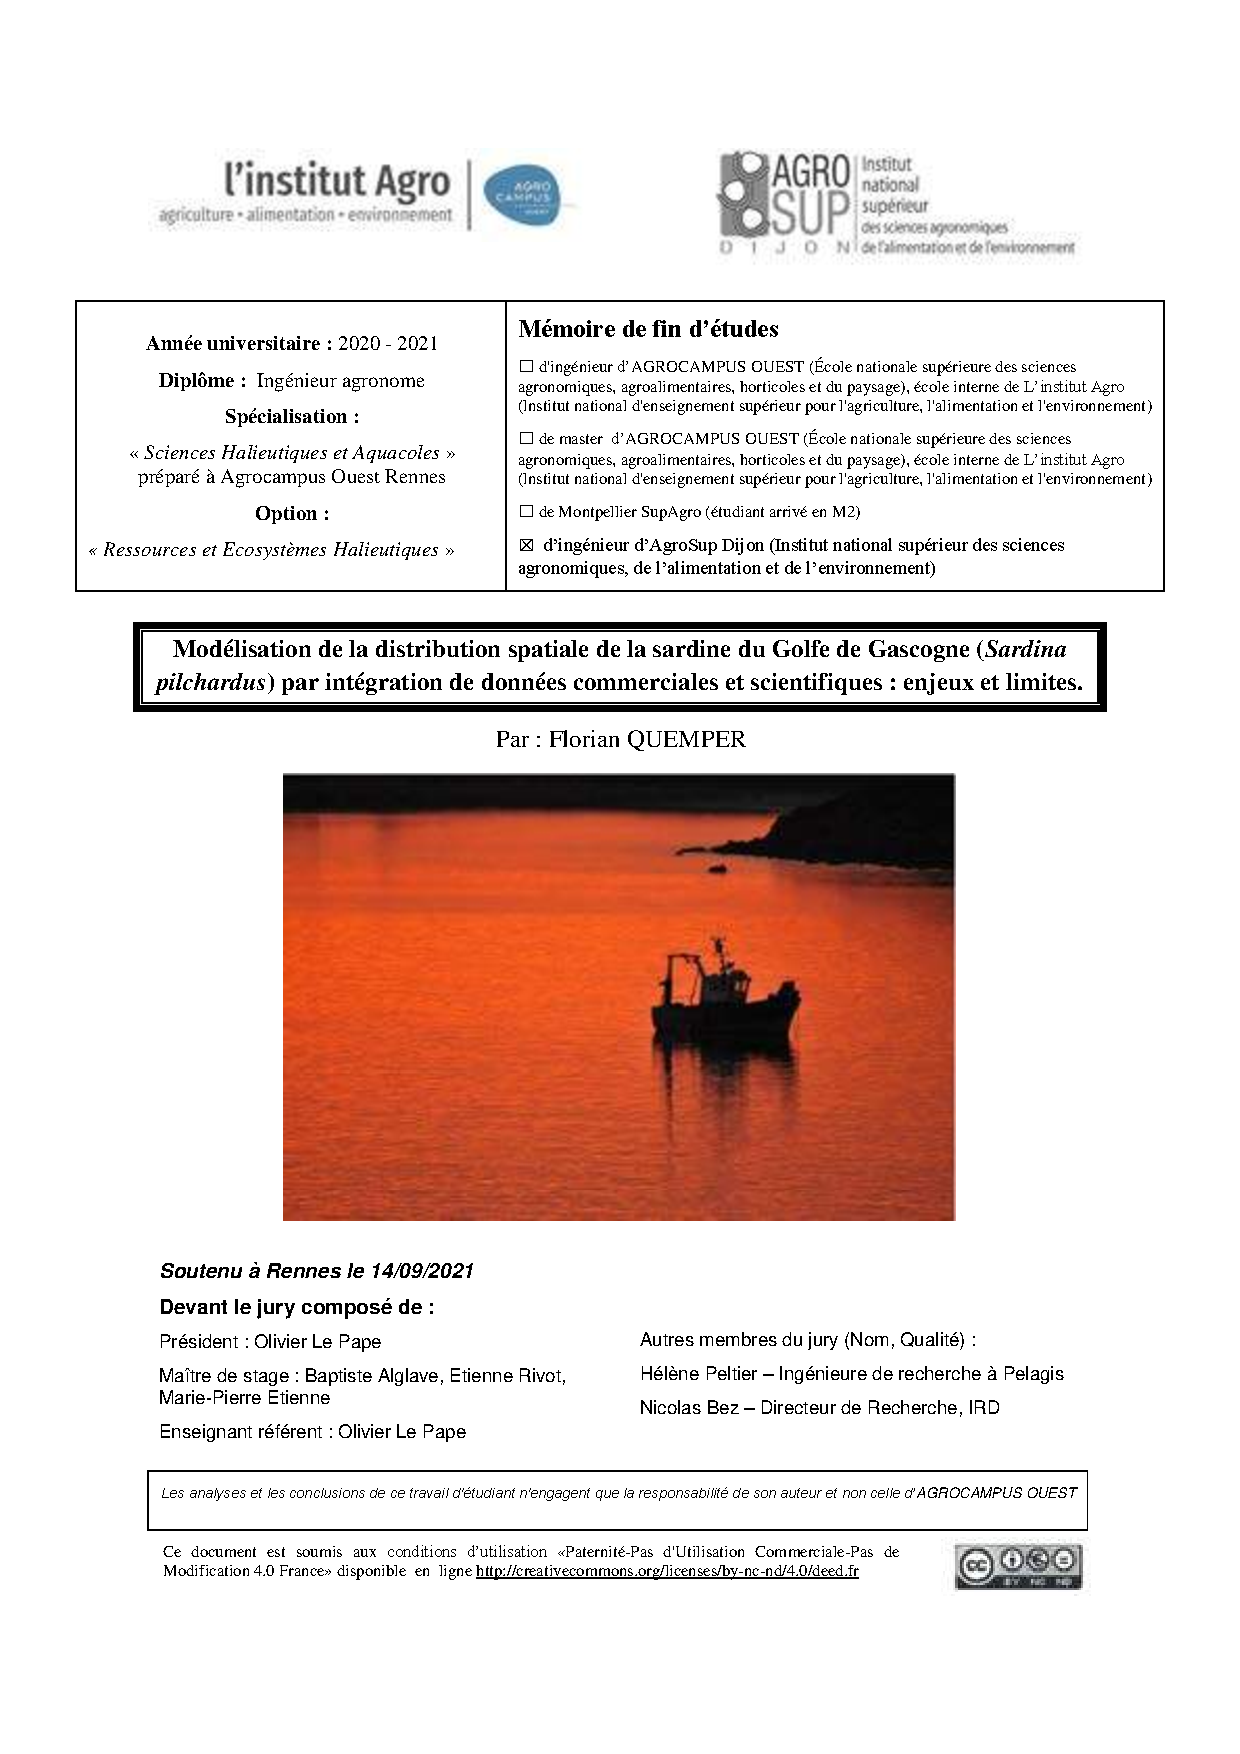
\includepdf[pages=-,pagecommand={},width=\textwidth]{Appendices/report/quemperstage.pdf}

\newpage

\section{Report of the ad-hoc contract for the preparation of STECF EWG 22-01 concerning closure areas to protect juveniles and spawners of all demersal stocks in western Mediterranean Sea}\label{appendix:STECFWG}


\includepdf[pages=-,pagecommand={},width=\textwidth]{Appendices/report/alglavevermardSTECF2191.pdf}

